 % arara: clean: { files: [thesis.aux, thesis.bbl, thesis.blg, thesis.dvi, thesis.fdb_latexmk, thesis.fls, thesis.idx, thesis.ilg, thesis.ind, thesis.lof, thesis.log, thesis.lot, thesis.nlo, thesis.nls, thesis.out, thesis.pdf, thesis.ps, thesis.toc]}
% arara: latex:  { shell: yes }
% arara: bibtex
% arara: nomencl
% arara: latex
% arara: makeindex
% arara: latex:  { shell: yes }
% arara: dvips
% arara: ps2pdf

% ******************************* PhD Thesis Template **************************
% Please have a look at the README.md file for info on how to use the template

\documentclass[a4paper,12pt,times,numbered,print,chapter]{Classes/PhDThesisPSnPDF}

% ******************************************************************************
% ******************************* Class Options ********************************
% *********************** See README for more details **************************
% ******************************************************************************

% `a4paper'(The University of Cambridge PhD thesis guidelines recommends a page
% size a4 - default option) or `a5paper': A5 Paper size is also allowed as per
% the Cambridge University Engineering Deparment guidelines for PhD thesis
%
% `11pt' or `12pt'(default): Font Size 10pt is NOT recommended by the University
% guidelines
%
% `oneside' or `twoside'(default): Printing double side (twoside) or single
% side.
%
% `print': Use `print' for print version with appropriate margins and page
% layout. Leaving the options field blank will activate Online version.
%
% `index': For index at the end of the thesis
%
% `draft': For draft mode without loading any images (same as draft in book)
%
% `draftmode': Special draft mode with line numbers, images, and water mark with
% timestamp and custom text. Position of the text can also be modified.
%
% `abstract': To generate only the title page and abstract page with
% dissertation title and name, to submit to the Student Registry
%
% `chapter`: This option enables only the specified chapter and it's references
%  Useful for review and corrections.
%
% ************************* Custom Page Margins ********************************
%
% `custommargin`: Use `custommargin' in options to activate custom page margins,
% which can be defined in the preamble.tex. Custom margin will override
% print/online margin setup.
%
% *********************** Choosing the Fonts in Class Options ******************
%
% `times' : Times font with math support. (The Cambridge University guidelines
% recommend using times)
%
% `fourier': Utopia Font with Fourier Math font (Font has to be installed)
%            It's a free font.
%
% `customfont': Use `customfont' option in the document class and load the
% package in the preamble.tex
%
% default or leave empty: `Latin Modern' font will be loaded.
%
% ********************** Choosing the Bibliography style ***********************
%
% `authoryear': For author-year citation eg., Krishna (2013)
%
% `numbered': (Default Option) For numbered and sorted citation e.g., [1,5,2]
%
% `custombib': Define your own bibliography style in the `preamble.tex' file.
%              `\RequirePackage[square, sort, numbers, authoryear]{natbib}'.
%              This can be also used to load biblatex instead of natbib
%              (See Preamble)
%
% **************************** Choosing the Page Style *************************
%
% `default (leave empty)': For Page Numbers in Header (Left Even, Right Odd) and
% Chapter Name in Header (Right Even) and Section Name (Left Odd). Blank Footer.
%
% `PageStyleI': Chapter Name next & Page Number on Even Side (Left Even).
% Section Name & Page Number in Header on Odd Side (Right Odd). Footer is empty.
%
% `PageStyleII': Chapter Name on Even Side (Left Even) in Header. Section Number
% and Section Name in Header on Odd Side (Right Odd). Page numbering in footer


% ********************************** Preamble **********************************
% Preamble: Contains packages and user-defined commands and settings
% ******************************************************************************
% ****************************** Custom Margin *********************************

% Add `custommargin' in the document class options to use this section
% Set {innerside margin / outerside margin / topmargin / bottom margin}  and
% other page dimensions
\ifsetCustomMargin
  \RequirePackage[left=37mm,right=30mm,top=35mm,bottom=30mm]{geometry}
  \setFancyHdr % To apply fancy header after geometry package is loaded
\fi

% *****************************************************************************
% ******************* Fonts (like different typewriter fonts etc.)*************

% Add `customfont' in the document class option to use this section

\ifsetCustomFont
  % Set your custom font here and use `customfont' in options. Leave empty to
  % load computer modern font (default LaTeX font).
  \RequirePackage{helvet}
\fi

% *****************************************************************************
% **************************** Custom Packages ********************************

% ************************* Algorithms and Pseudocode **************************

%\usepackage{algpseudocode}
\usepackage{listings}

% ********************Captions and Hyperreferencing / URL **********************

% Captions: This makes captions of figures use a boldfaced small font.
%\RequirePackage[small,bf]{caption}

\RequirePackage[labelsep=space,tableposition=top]{caption}
\renewcommand{\figurename}{Fig.} %to support older versions of captions.sty


% *************************** Graphics and figures *****************************

%\usepackage{rotating}
\usepackage{wrapfig}

% Uncomment the following two lines to force Latex to place the figure.
% Use [H] when including graphics. Note 'H' instead of 'h'
%\usepackage{float}
%\restylefloat{figure}

% Subcaption package is also available in the sty folder you can use that by
% uncommenting the following line
% This is for people stuck with older versions of texlive
%\usepackage{sty/caption/subcaption}
\usepackage{subcaption}


% ********************************** Tables ************************************
\usepackage{booktabs} % For professional looking tables
\usepackage{multirow}

%\usepackage{multicol}
%\usepackage{longtable}
%\usepackage{tabularx}


% ***************************** Math and SI Units ******************************

\usepackage{amsfonts}
\usepackage{amsmath}
\usepackage{amssymb}
\usepackage{siunitx} % use this package module for SI units
\usepackage[euler]{textgreek}

% ******************************* Line Spacing *********************************

% Choose linespacing as appropriate. Default is one-half line spacing as per the
% University guidelines

%\doublespacing
%\onehalfspacing
\singlespacing


% ************************ Formatting / Footnote *******************************

% Don't break enumeration (etc.) across pages in an ugly manner (default 10000)
%\clubpenalty=500
%\widowpenalty=500

%\usepackage[perpage]{footmisc} %Range of footnote options


% *****************************************************************************
% *************************** Bibliography  and References ********************

%\usepackage{cleveref} %Referencing without need to explicitly state fig /table

% Add `custombib' in the document class option to use this section
\ifuseCustomBib
   \RequirePackage[square, sort, numbers, authoryear]{natbib} % CustomBib

% If you would like to use biblatex for your reference management, as opposed to the default `natbibpackage` pass the option `custombib` in the document class. Comment out the previous line to make sure you don't load the natbib package. Uncomment the following lines and specify the location of references.bib file

%\RequirePackage[backend=biber, style=numeric-comp, citestyle=numeric, sorting=nty, natbib=true]{biblatex}
%\bibliography{References/references} %Location of references.bib only for biblatex

\fi

% changes the default name `Bibliography` -> `References'
\renewcommand{\bibname}{References}


% *****************************************************************************
% *************** Changing the Visual Style of Chapter Headings ***************
% This section on visual style is from https://github.com/cambridge/thesis

% Uncomment the section below. Requires titlesec package.

%\RequirePackage{titlesec}
%\newcommand{\PreContentTitleFormat}{\titleformat{\chapter}[display]{\scshape\Large}
%{\Large\filleft{\chaptertitlename} \Huge\thechapter}
%{1ex}{}
%[\vspace{1ex}\titlerule]}
%\newcommand{\ContentTitleFormat}{\titleformat{\chapter}[display]{\scshape\huge}
%{\Large\filleft{\chaptertitlename} \Huge\thechapter}{1ex}
%{\titlerule\vspace{1ex}\filright}
%[\vspace{1ex}\titlerule]}
%\newcommand{\PostContentTitleFormat}{\PreContentTitleFormat}
%\PreContentTitleFormat


% ******************************************************************************
% ************************* User Defined Commands ******************************
% ******************************************************************************

% *********** To change the name of Table of Contents / LOF and LOT ************

%\renewcommand{\contentsname}{My Table of Contents}
%\renewcommand{\listfigurename}{My List of Figures}
%\renewcommand{\listtablename}{My List of Tables}

\lstdefinestyle{haskellStyle}{
	language=Haskell,
	numbers=left,
	stepnumber=1,
	numbersep=10pt,
	tabsize=4,
	showspaces=false,
	showstringspaces=false,
	basicstyle=\footnotesize,
	columns=flexible
}
\newcommand{\vecb}[1]{\vec{\mathbf{#1}}}
\newcommand{\matr}[1]{\mathbf{#1}}
\newcommand{\code}[1]{\lstinline{#1}}
\newcommand{\sep}{\hspace{50pt}}
\newcommand{\clash}{C$\lambda$aSH}
\newcommand{\matlab}{MATLAB} %\textsuperscript{\textregistered}
\providecommand{\e}[1]{\ensuremath{\times 10^{#1}}}

\newenvironment{itemizens}
{ 
	\vspace{-\topsep}
	\begin{itemize}
	\setlength{\itemsep}{0pt}
	\setlength{\parskip}{0pt}
	\setlength{\parsep}{0pt}     
}
{ 
	\end{itemize}
} 

\newenvironment{enumeratens}
{
	\vspace{-\topsep}
	\begin{enumerate}
	\setlength{\itemsep}{0pt}
	\setlength{\parskip}{0pt}
	\setlength{\parsep}{0pt}     
}
{ 
	\end{enumerate}                  
} 


% ********************** TOC depth and numbering depth *************************

\setcounter{secnumdepth}{2}
\setcounter{tocdepth}{2}


% ******************************* Nomenclature *********************************

% To change the name of the Nomenclature section, uncomment the following line

%\renewcommand{\nomname}{Symbols}


% ********************************* Appendix ***********************************

% The default value of both \appendixtocname and \appendixpagename is `Appendices'. These names can all be changed via:

%\renewcommand{\appendixtocname}{List of appendices}
%\renewcommand{\appendixname}{Appndx}

% ******************************** Draft Mode **********************************

% Uncomment to disable figures in `draftmode'
%\setkeys{Gin}{draft=true}  % set draft to false to enable figures in `draft'

% These options are active only during the draft mode
% Default text is "Draft"
%\SetDraftText{DRAFT}

% Default Watermark location is top. Location (top/bottom)
%\SetDraftWMPosition{bottom}

% Draft Version - default is v1.0
%\SetDraftVersion{v1.1}

% Draft Text grayscale value (should be between 0-black and 1-white)
% Default value is 0.75
%\SetDraftGrayScale{0.8}


%% Todo notes functionality
%% Uncomment the following lines to have todonotes.

%\ifsetDraft
%	\usepackage[colorinlistoftodos]{todonotes}
%	\newcommand{\mynote}[1]{\todo[author=kks32,size=\small,inline,color=green!40]{#1}}
%\else
%	\newcommand{\mynote}[1]{}
%	\newcommand{\listoftodos}{}
%\fi

% Example todo: \mynote{Hey! I have a note}


% ************************ Thesis Information & Meta-data **********************
% Thesis title and author information, refernce file for biblatex
% ************************ Thesis Information & Meta-data **********************
%% The title of the thesis
\title{Numerical mathematics on FPGAs using C\textlambda aSH}
%\texorpdfstring is used for PDF metadata. Usage:
%\texorpdfstring{LaTeX_Version}{PDF Version (non-latex)} eg.,
%\texorpdfstring{$sigma$}{sigma}

%% Subtitle (Optional)
\subtitle{Comparison to conventional solution methods}

%% The full name of the author
\author{Martijn Bakker}

%% Department (eg. Department of Engineering, Maths, Physics)
\dept{Committee: \\ 
	Dr.ir. J. Kuper \\ 
	Dr. R.M.J. van Damme \\ 
	Dr.ir. J. Broenink \\ 
	\vspace{150pt}	
	Computer Architecture for Embedded Systems
	Electrical Engineering, Mathematics and Computer Science (EEMCS)
}

%% University and Crest
\university{University of Twente}
%\crest{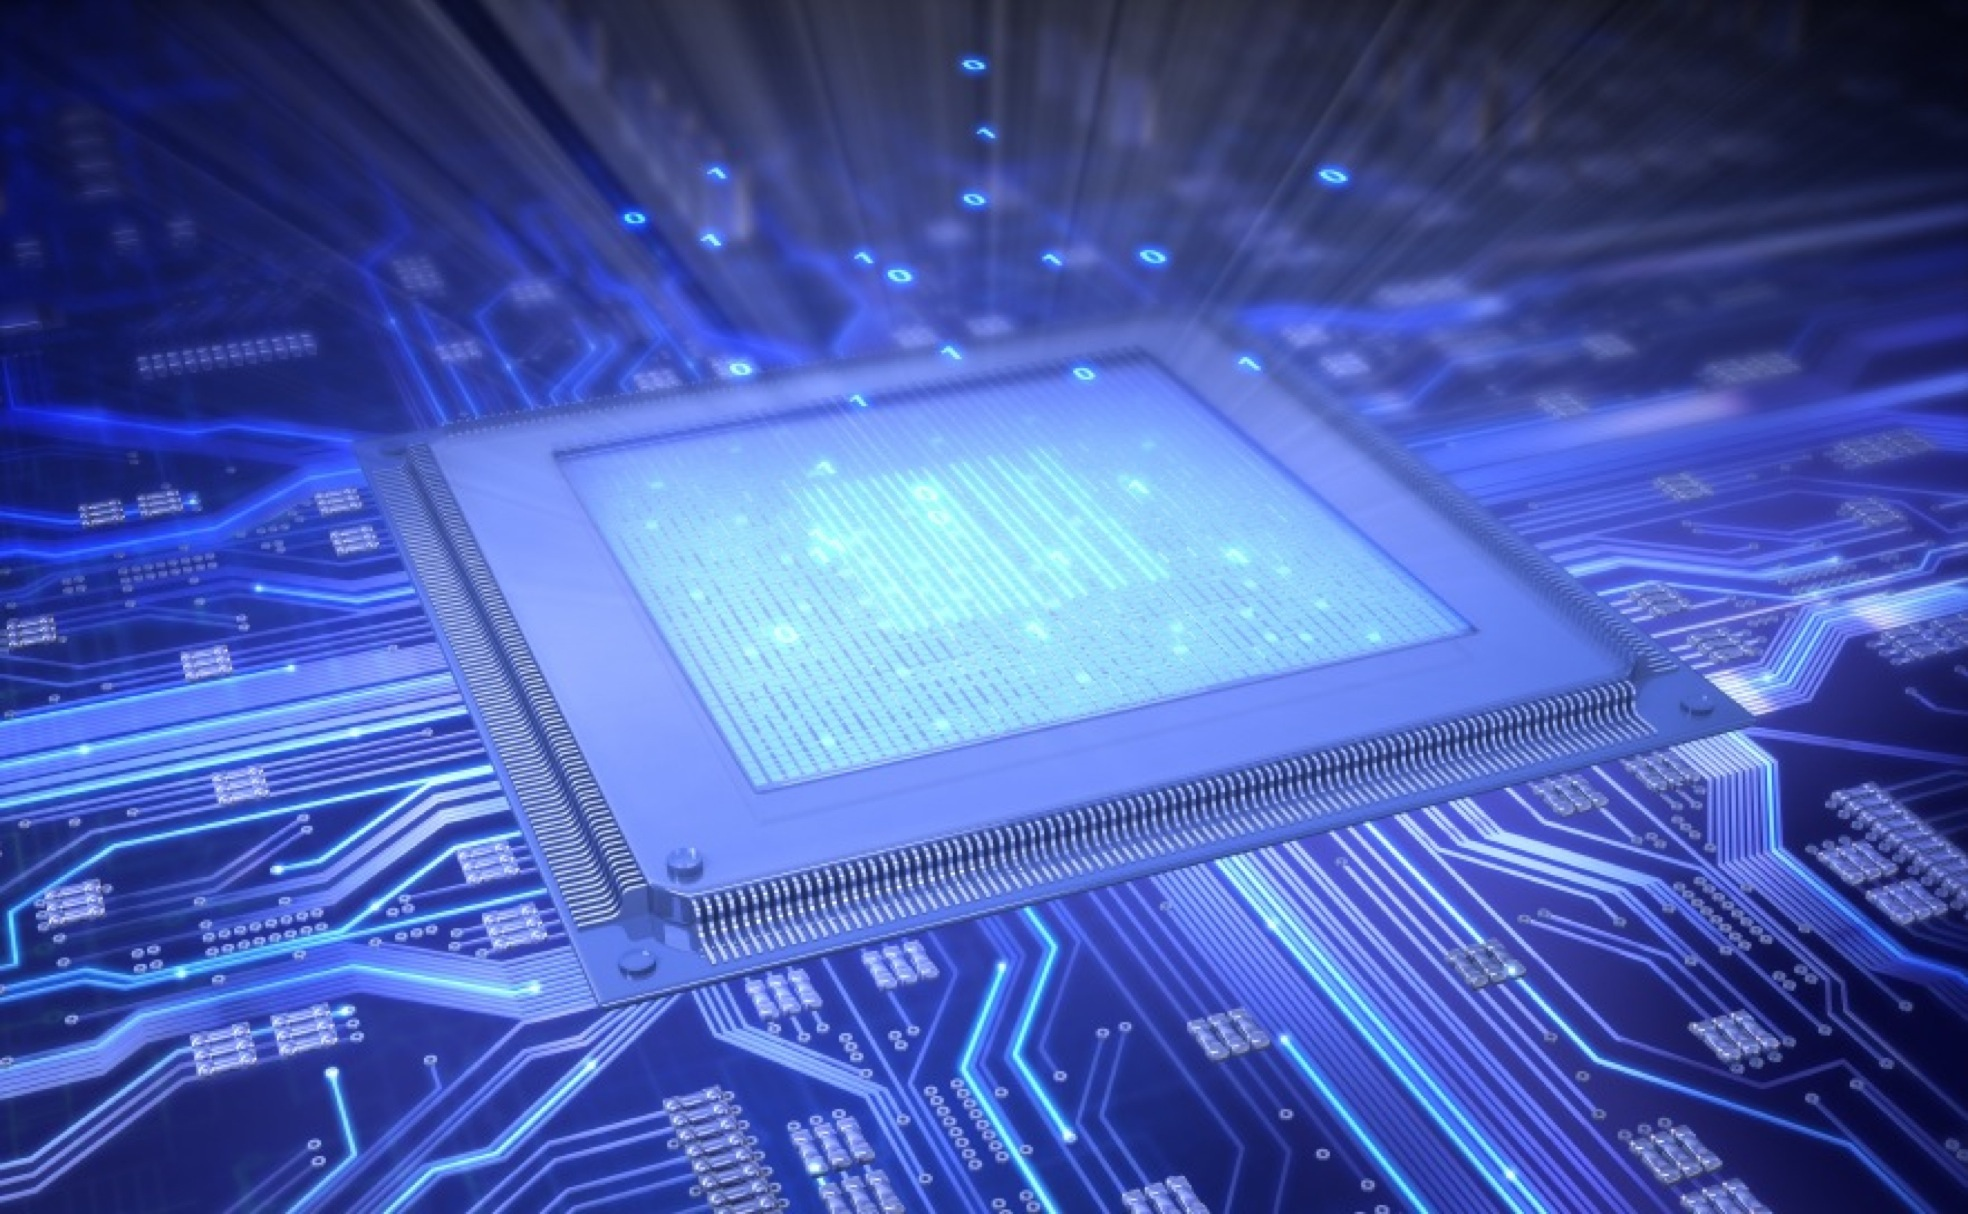
\includegraphics[width=\textwidth]{fpga_wallpaper}}

%% You can redefine the submission text:
% Default as per the University guidelines:
% ``This dissertation is submitted for the degree of''
\renewcommand{\submissiontext}{This thesis is submitted for the degree of}

%% Full title of the Degree
\degreetitle{Bachelor of Science}

%% College affiliation (optional)
\college{Advanced Technology}

%% Submission date
% Default is set as {\monthname[\the\month]\space\the\year}
\degreedate{July 2015} 

%% Meta information
\subject{LaTeX} \keywords{{LaTeX} {PhD Thesis} {Engineering} {University of Cambridge}}


% ***************************** Abstract Separate ******************************
% To printout only the titlepage and the abstract with the PhD title and the
% author name for submission to the Student Registry, use the `abstract' option in
% the document class.
\ifdefineAbstract
 \pagestyle{empty}
 \includeonly{Declaration/declaration, Abstract/abstract}
\fi

% ***************************** Chapter Mode ***********************************
% The chapter mode allows user to only print particular chapters with references
% Title, Contents, Frontmatter are disabled by default
% Useful option to review a particular chapter or to send it to supervisior.
% To use choose `chapter' option in the document class
\ifdefineChapter
 \includeonly{P1-Introduction/introduction}
\fi

% ******************************** Front Matter ********************************
\begin{document}

\frontmatter

\begin{titlepage}
  \maketitle
\end{titlepage}

% ************************** Thesis Acknowledgements **************************

\begin{acknowledgements}      
\begin{itemizens}
	\item Jan Kuper	- Introducing me to functional programming, \clash{} and giving feedback
	\item Christiaan Baaij - Creating \clash{} and answering related questions
	\item Ruud van Damme \& Jan Broenink - Feedback
	\item Rinse Wester - Input on configuring and using the Avalon bridges
\end{itemizens}

\end{acknowledgements}


\vfill

\begin{acronyms}
\begin{tabular}{>{\bfseries}l l}
	ASIC & Application-specific integrated circuit \\
	FPGA & Field-Programmable Gate Array \\
	CPU & Central Processing Unit \\
	%GPU & Graphics Processing Unit \\
	%GPGPU & General Purpose GPU \\
	DSP & Digital Signal Processing \\
	LED & Light Emitting Diode \\
	VHDL & VHSIC HDL \\
	VHSIC & Very High Speed Integrated Circuit \\
	HDL & Hardware Description Language \\
	SoC & System-on-Chip \\ 
	ODE & Ordinary Differential Equation \\
	HPS & Hard Processor System \\
	ARM & Advanced RISC Machine (CPU development company) \\
	RISC & Reduced Instruction Set Computer \\
	IP & Intellectual Property \\
	GUI & Graphical User Interface \\
\end{tabular}		
\end{acronyms}    

  

\begin{abstract}
Performing computations directly in hardware can be a very challenging task for a scientist or engineer only familiar with software, but there is much that can be gained in terms of power reduction and performance improvements using FPGAs. This thesis describes the process of implementing an accelerator in which the computational part is specified using the functional hardware description language \clash{} and discusses the feasibility of performing numerical mathematics on this accelerator by computing approximations to ordinary differential equations. The accelerator is capable of using the methods of Euler and Runge-Kutta (second order) to perform the approximations, but due to the use of a fixed-point number representation the accuracy suffers. The performance of the accelerator, implemented on a low-power, low-cost development FPGA: the Altera Cyclone V is 40\% worse than an i7-950, but the power usage of the accelerator is 2 orders of magnitude lower. 
\end{abstract}


% *********************** Adding TOC and List of Figures ***********************

\tableofcontents
\listoffigures
\listoftables

% \printnomencl[space] space can be set as 2em between symbol and description
%\printnomencl[3em]

\printnomencl

% ******************************** Main Matter *********************************
\mainmatter


\chapter{Introduction} 

\section{Solver theory -- TODO}

\subsubsection{Euler}
Take derivative, multiply with timestep, add to initial value, repeat until end.

\subsubsection{Runge-Kutta methods}
Take derivatives at some time points, multiply with proper coefficients, add all to intial value, repeat until end.

\subsubsection{Stability}

\section{What is FP -- TODO}
Should I add a section on this to make everything understandable to all readers?


\section{Using Haskell for numerical mathematics}
Functional languages have several properties which make them suitable for the purpose of solving problems in numerical mathematics. First and foremost, Haskell, being based on $\lambda$-calculus is very close to mathematics. The useful mathematical properties here are \textit{referential transparency}, easy \textit{partial function application} and being a \textit{declarative language}. 
Referential transparency implies that a variable only has a constant value which is the same everywhere in the program. This prevents that changing a variable might have influence on another computation as a side effect and it corresponds to mathematical notation. For instance, in an imperative programming like C you could write \code{i = i + 1}, which is a mathematical impossibility and therefore not allowed in Haskell. 
Partial function application is another very useful concept. Often in numerical mathematics, you want to create or process a function. You need a function that has another function as return value. For instance, take a function which requires two arguments. After only applying a single argument, the object returned still needs the second argument in order to compute the final value. This is exactly according to the definition of a function: An object that still needs arguments before being able to return its final value.
Being a \textit{declarative language} means that you write code that specifies what you want to accomplish, not how to get there. This concept is again borrowed from mathematics. You put in a set of function definitions and Haskell will figure out how to actually compute the value you request according to those definitions. This property of declarativity also has the result that Haskell is a very terse language whilst remaining easy to understand.
Secondly, Haskell has a very strong type system. The type system has three main advantages. It becomes very easy to swap out and replace functions as long as you make sure that the types are the same. The Haskell compiler will start to assert errors immediately whenever you feed it something which does not make sense or could be ambiguous which is very useful when writing programs. By having a look at the types of a Haskell program it becomes very straightforward to see what the program does and how it works, which is very useful when attempting to understand your own or someone else's code.
Lastly, a property which is often very important for numerical mathematics: Haskell is fast. According to the \textit{Computer Language Benchmarks Game} \cite{Bench}, Haskell is almost on par with Java and Fortran but significantly faster than Python and Matlab (not shown), two languages which are often used for numerical mathematics nowadays. There is still a performance gap of around a factor 3 between Haskell and C (the reference), hence if speed is of the absolute highest concern C is still a valid option.

\section{Numerical solutions of ODEs in Haskell}
\lstset{style=haskellStyle}

As mentioned before, the types in Haskell reveal lots of information about the structure and functionality of the program. The three main types constituting the numerical solver for ordinary differential equations are listed above.

\lstinputlisting[caption=Main types for the ODE solver, label=solvertypes, firstline=18]{../haskell/SolverTypes.hs}

\subsubsection{Equation}
In essence, a differential equation is a mapping (function) from a certain state of the system to the change of this system. This is also what the type signature of \code{Equation} signifies, a mapping from an \code{ODEState} to a \code{D_ODEState}. This generic set up allows the specification of any ODE for solving. The implementation in pure Haskell of a simple ODE is given in listing \ref{lst:eq_exponential}, which corresponds to the equation $x' = -x$. However, this representation is not very elegant and a lot of the code is performing unboxing of the types. Using property that this equation is linear, it is possible to use an utility method which takes as input a matrix and returns the Haskell differential equation function belonging to that matrix. The same can be done for heterogeneous linear systems using a different utility function, which does not only takes a matrix as input but also a list of functions representing the heterogeneous part of the equation. The example code for this can be seen in appendix \ref{app:haskellsolver}.

\lstinputlisting[caption=Example equation for exponential decay, label=lst:eq_exponential, firstline=11,lastline=14]{../haskell/SolverEquations.hs}

\subsubsection{SolveMethod}
The \code{SolveMethod} performs the actual computations on what the next value of the solution should be: the integration scheme. In order to obtain this next state, the scheme needs three input values: It needs information on the timing constraints of the solution, in this case it needs the time step. Furthermore, it needs the equation itself and it requires the state of the system at $t_{n}$ in order to be able to determine the state of the system at $t_{n+1} = t_{n} + \Delta t$.

The most straightforward integration scheme is called forward Euler, given in equation \ref{eq:forward_euler}. Listing \ref{lst:forward_euler} depicts the translation of the mathematical expression \ref{eq:forward_euler} to Haskell. Even though some list operations have been inserted (\code{zipWith} and \code{map}), the structure is still recognizable. It computes the change in state, multiplies this with the time step obtained in line 6 and adds the initial state in line 4. Lastly, the integration scheme returns the new state of the equation, consisting of a list of x-values and a corresponding time value. Implementations of different solvers (eg. 4th order Runge-Kutta) can be found in appendix \ref{app:haskellsolver}.

\lstinputlisting[caption=Example code for the forward Euler integration scheme, label=lst:forward_euler, firstline=9,lastline=15]{../haskell/SolverSolvers.hs}

\begin{equation}
\label{eq:forward_euler}
\vecb{x}(t + \Delta t) \approx \vecb{x}(t) + \frac{\mathrm d \vecb{x}(t)}{\mathrm d t}\Delta t
\end{equation}

\subsubsection{Solver}
The \code{Solver} function in listing \ref{lst:solver_frame} acts as the main interface to the program. You specify a \code{SolveMethod}, the \code{TimeSettings} (containing the time step and the time at which to stop solving), the equation itself and an initial condition. The \code{Solver} will then return a list of states of the system. As is very common in functional programming, the \code{Solver} has been defined recursively. Line 4 is where the magic happens: the solution list is defined to be the initial condition, followed by the solution list with the new state (computed by the integration scheme on line 6) as initial condition. Additionally, there is a comparison in line 7 which ends the recursion whenever the time of the solution exceeds the maximum time value, set in the \code{TimeSettings}.

The solutions of a wide range of equations, both linear and non-linear, both homogeneous and heterogeneous and using the input matrix utility functions have been plot with suitable initial conditions to show their behavior in figure \ref{fig:solver_example}.

\lstinputlisting[caption=The main controlling function, label=lst:solver_frame, firstline=14,lastline=20]{../haskell/Solver.hs}

\begin{figure}[h!]
	\centering
	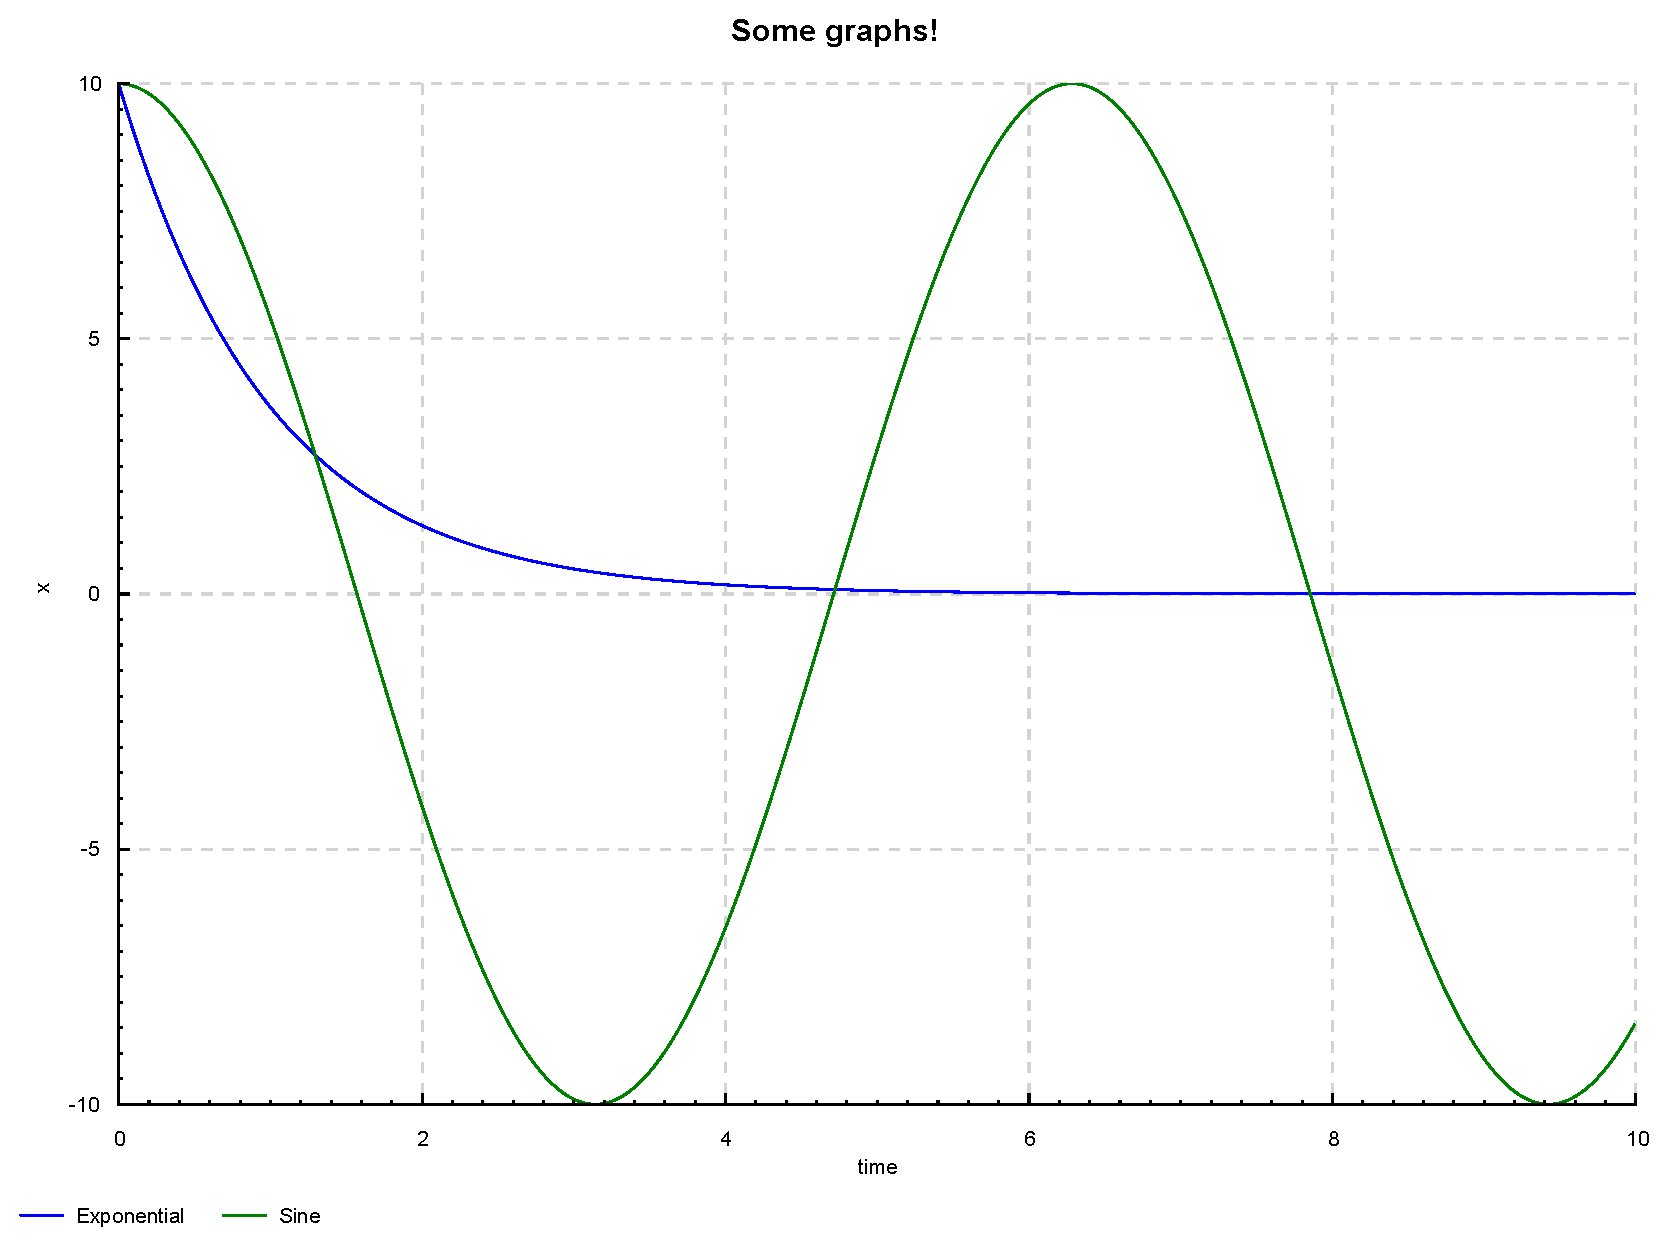
\includegraphics[width=\textwidth]{../haskell/output.pdf}
	\caption{Graphs}
	\label{fig:solver_example}
\end{figure}

\begin{align}
\text{Exponential}\sep{}			x(t)' &= -x(t)  \\
\text{Simple harmonic}\sep{}		x(t)'' &= -x(t) \\
\text{Cosine hyperbolic}\sep{}		x(t)' &= \frac{\sqrt{x(t)^{2} - a^{2}}}{a} \\
\text{Simple harmonic}\sep{}		\vecb{x}(t)' &= \begin{bmatrix} 0 & 1 \\ -1 & 0 \\ \end{bmatrix}\vecb{x}(t) \\
\text{Simple forced harmonic}\sep{}	\vecb{x}(t)' &= \begin{bmatrix} 0 & 1 \\ -1 & 0 \\ \end{bmatrix}\vecb{x}(t) + \begin{bmatrix} \sin{(t)} \\ e^{-t} \\ \end{bmatrix}
\end{align}




\section{Conversion to Mealy Machines / C$\lambda$aSH -- TODO}

Changes to:
\begin{itemize}
	\item Equation : numerical types (fixed point) - what operations would be supported in VHDL (hard to do nonlinear operators, sqrt(), sin(), cos(), tan()) - 
	\item SolutionMethod - becomes transition function of the mealy machine
	\item Solver - keeping track of the state of the solution - responsible for loading the data from the AXI-bridge to the HPS - responsible for outputting the data to the HPS for storage/processing/streaming
\end{itemize}

\iffalse
\begin{equation}
\frac{\mathrm d \vecb{x}(t)}{\mathrm d t} = f(\vecb{x}) + g(t)
\end{equation}

\begin{equation}
\frac{\mathrm d \vecb{x}(t)}{\mathrm d t} = \matr{A} \vec{x} + g(t)
\end{equation}
\fi

\section{FPGAs -- TODO}
\begin{itemize}
	\item What are FPGAs used for?
	\item Why should I care about FPGAs
	\item What is the current workflow for programming FPGAs
\end{itemize}


\section{Data transfer -- TODO}
\chapter{Results}
\label{s:results}

\section{Euler}
One of the first tests for an ODE solver is whether it handles harmonic oscillations properly. The simple oscillations (shown in \ref{eq:osceq} with their analytical solutions) can be implemented as a matrix vector equation (\ref{eq:oscmatrix}), which represents two uncoupled oscillations of different frequencies. Besides the matrix of constants, the solver also requires initial values. For the first oscillation the initial position is non-zero, for the second oscillation the initial velocity is non-zero. 

\begin{align}
\label{eq:osceq} \nonumber
x_{0} '' &= - x_{0} \\
x_{2} '' &= -4 x_{2} \\ \nonumber
\\ \nonumber
\label{eq:osceqsol} \nonumber
x_{0}(t)  &= 50 \cos{(t)} \\ \nonumber
x_{2}(t)  &= 25 \sin{(2t)} \\ \nonumber
\end{align}


\begin{equation}
\label{eq:oscmatrix}
\vecb{x}' = \begin{bmatrix} 
0 & 1 & 0 & 0 \\
-1 & 0 & 0 & 0 \\
0 & 0 & 0 & 1 \\
0 & 0 & -4 & 0 \\
\end{bmatrix} \vecb{x} 
\hspace{20pt} \text{with} \hspace{20pt} 
\vecb{x}(t = 0) =\begin{bmatrix} 50 \\ 0 \\ 0 \\ 50 \end{bmatrix} 
\end{equation}


\begin{figure}[h]
	\centering
	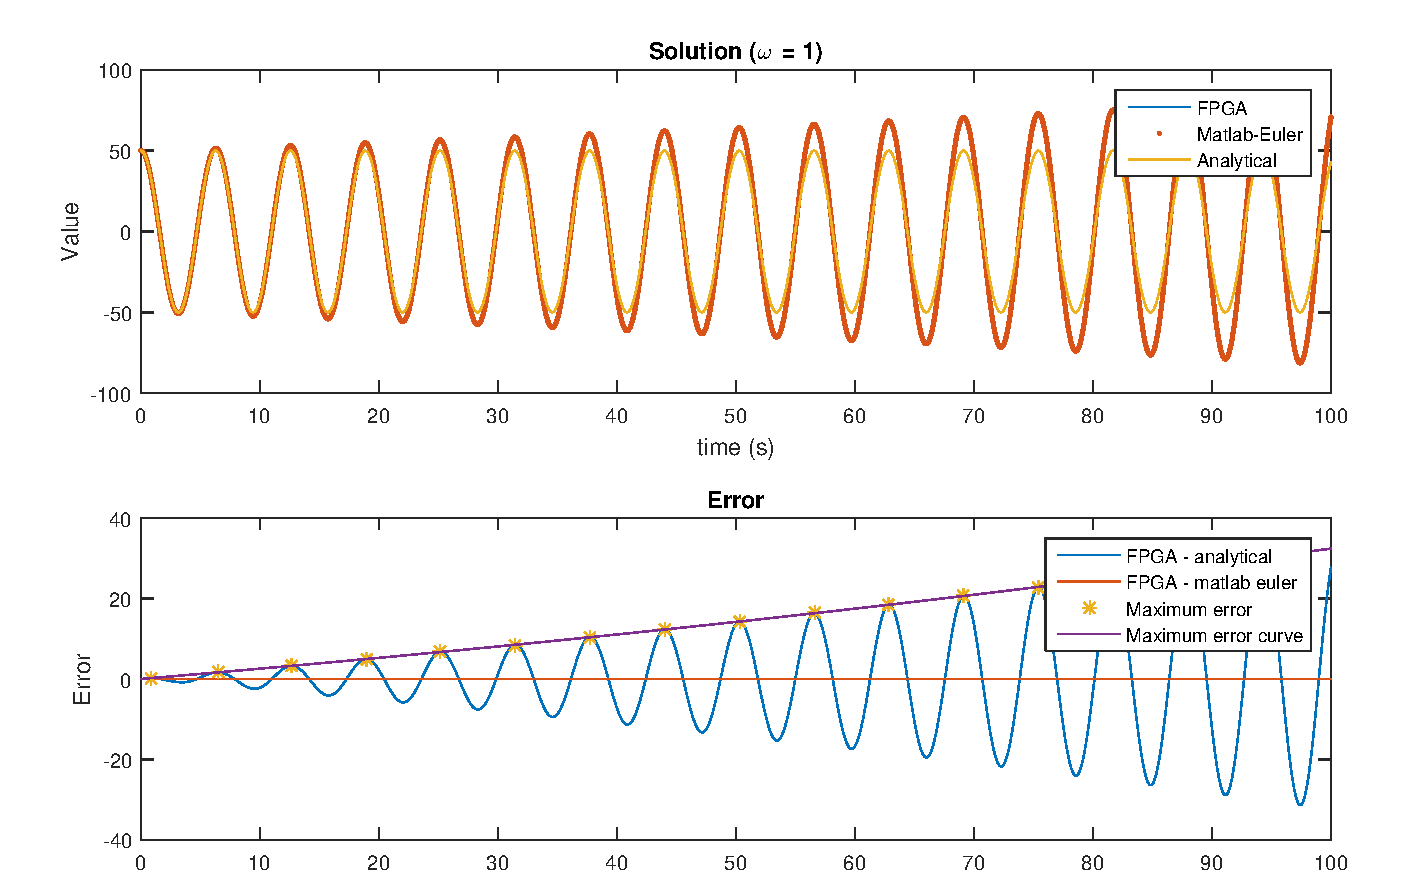
\includegraphics[width=\textwidth]{euler_o1_ts=0,01_os=1}
	\caption{Simple oscillation using Euler's method (h = 0.01)}
	\label{f:euler_o1_ts=0,01_os=1}
\end{figure}

\subsection{First oscillation - initial position}
The plots belonging to the first oscillation (\ref{f:euler_o1_ts=0,01_os=1}) depict three variations on solving the system. Firstly, it contains the solution generated by the FPGA. Secondly, it contains the result of the exact same combination of equation and solver, but implemented in \matlab{}. The only difference between the FPGA and \matlab{} implementation is the number representation. Therefore, if the FPGA solution starts to diverge from the \matlab{} solution the reason has to be the reduced accuracy of the 32-bit fixed point representation used in the FPGA. Internally, \matlab{} uses a (64-bit) double precision floating format \cite{MatlabFloat}, which is guaranteeing a precision of ~15 significant figures for almost all magnitudes supported by the IEEE 754 double precision floating point standard. Lastly, the plot contains the analytical solution of the problem.

The plot shows that the FPGA exhibits the expected behaviour of solving a simple oscillation with Euler's method. Due to the relatively large step size (h = 0.01) the approximation quickly diverges from the analytical solution. The curvature of the solution is always opposite in sign to the solution itself ($x'' = -x$), which results in a self-amplifying effect in the magnitude of the error: an exponential error growth. This was expected, as the exponential dependency was already derived by \cite{DE} in equation \ref{eq:euler_error}. However, this does show that Euler's method is a particularly bad integration scheme for a simple oscillation. It is possible to use \matlab{}s Curve Fitting Tool to fit the equation of the theoretical maximum error of Euler's method to the points of maximum error. After combining some constants, \ref{eq:euler_error} becomes equal to \ref{eq:euler_error_combined}. For $a = 49.75$ and $b = 0.00502$ this equation achieves a fit of $R^{2} = 1$, which is a perfect fit. The error plot and the curve fit of the maximum errors are shown in \ref{f:euler_o1_ts=0,01_os=1}.

\begin{equation}
\label{eq:euler_error_combined}
\text{error}_{\text{euler}}(t) = a (e^{b t} - 1)
\end{equation}

Lastly, the FPGA solution the solution of Euler's method implemented in \matlab{} shows that the error due to the fixed point number representation is clearly insignificant when compared to the intrinsic error in Euler's method: the maximum absolute difference between the two solutions is less than 6\e{-5}.

\subsubsection{Decreasing the time step - improving accuracy?}
The expectation based on \cite{DE} and equation \ref{eq:euler_error} is that the maximum error is indeed proportional to the time step, meaning that a hundred fold decrease of the time step also decreases the error by a factor 100. The maximum error at $t \approx 100$ for $h = 0.01$ was $\approx 30$, whereas the maximum error for $h = 0.0001$ is $\approx 0.2$, which is an improvement of $150 \times$, 50\% more than expected. However, even though the error relative to the analytical solution has decreased, the divergence from the \matlab{} implementation of Euler's algorithm has increased to 8\e{-4}, a factor of 13.

As the time step gets decreased even more, eventually the improvement of having a shorter time step loses out to the reduction the accuracy in the computation. This can be seen very clearly in \ref{f:euler_o1_ts=0,0000001_os=1000}. Featuring a time step of h = 1 \e{-7}, which is approaching the smallest representable value at $2^{-24}$. In this case the \matlab{} implementation is still following the analytical solution with little whereas the solution generated by the FPGA begins to diverge noticeably.

\begin{figure}[h]
	\centering
	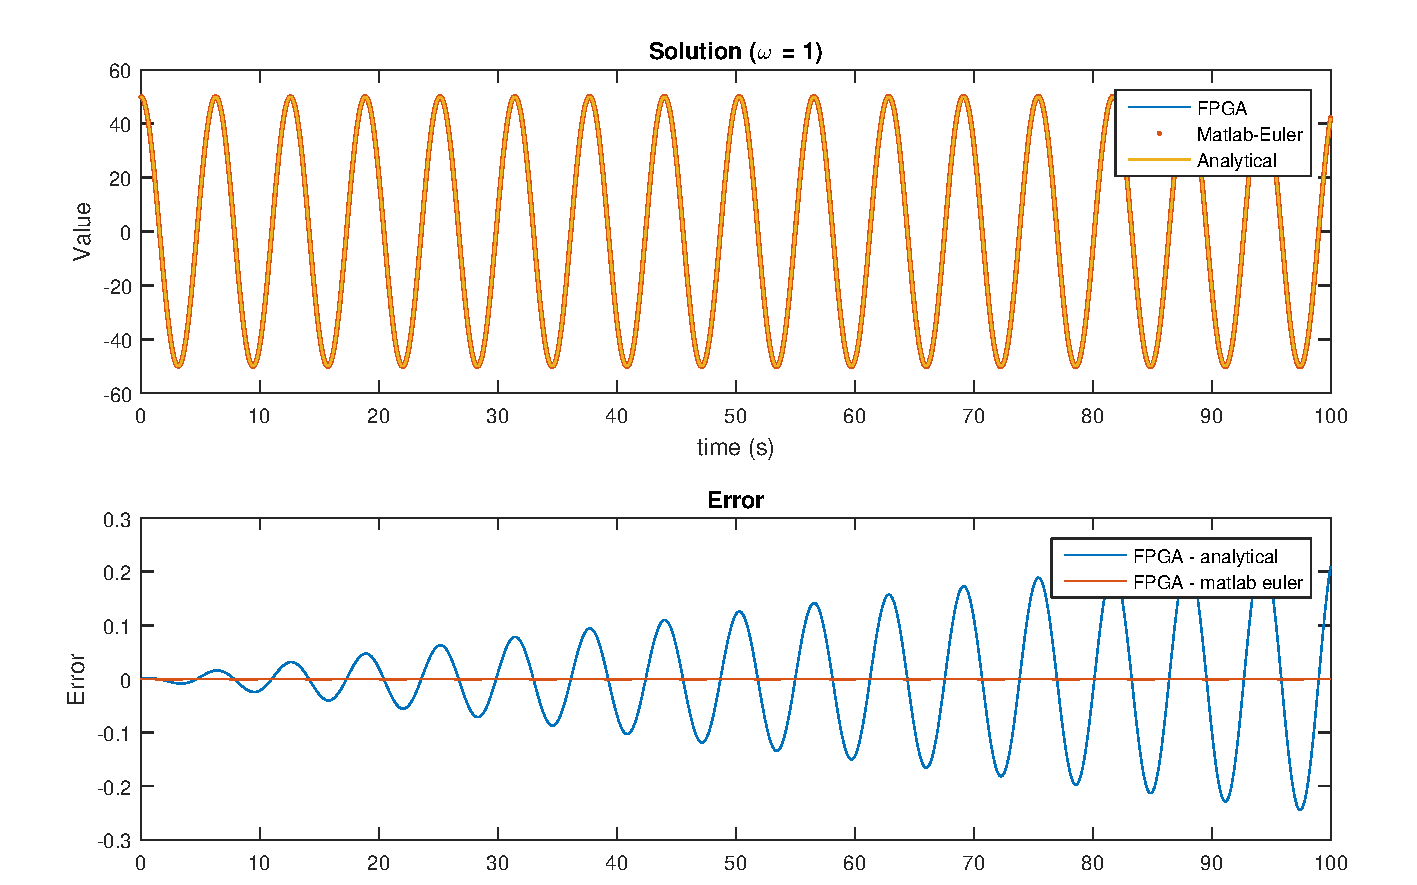
\includegraphics[width=\textwidth]{euler_o1_ts=0,0001_os=100}
	\caption{Simple oscillation using Euler's method with a lower time step (h = 1 \e{-4})}
	\label{f:euler_o1_ts=0,0001_os=100}
\end{figure}

\begin{figure}[h]
	\centering
	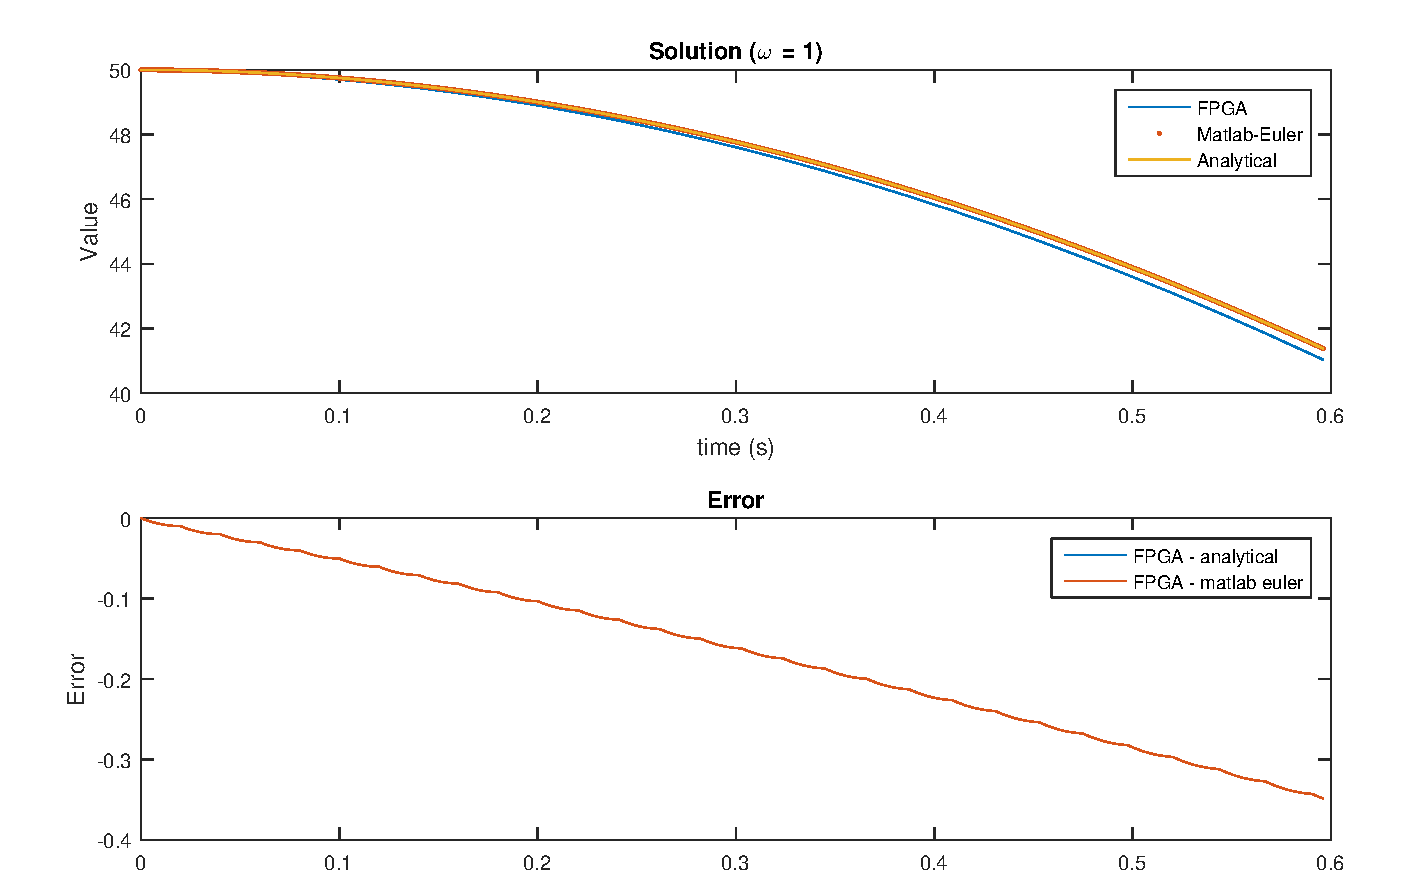
\includegraphics[width=\textwidth]{euler_o1_ts=0,0000001_os=1000}
	\caption{Approaching breakdown due to the fixed point number representation (h = 1 \e{-7})}
	\label{f:euler_o1_ts=0,0000001_os=1000}
\end{figure}

\subsection{Second oscillation - initial velocity}
Similarly to the previous scenario, the error increases exponentially over time and an decrease in time step is approximately proportional to the decrease in error (figure \ref{f:euler_o2_ts=0,001_os=100} and \ref{f:euler_o2_ts=0,00001_os=1000}). However, there is an important difference between the two oscillations: the frequency of oscillation is higher. This has as result that the time step of $h = 0.01$ which worked fine for the oscillation with $\omega = 1$ does not work properly any more: it results in figure \ref{f:euler_o2_ts=0,01_os=1}. This figure shows two interesting phenomena. Firstly, even though \matlab{}s Euler's method does diverge from the analytical solution, it only diverges in magnitude: it stays in phase. However, when looking at the FPGA solution you notice that it diverges from the other two, not only in magnitude but also in phase. The discrepancy in phase between \matlab{} and FPGA indicates that the number representation is the culprit of the shift. 

An attempt to fix this problem was made by changing the relevant part of the matrix from $\left[ \begin{smallmatrix} 0 & 1\\ -4 & 0 \end{smallmatrix} \right]$ to $\left[ \begin{smallmatrix} 0 & 2\\ -2 & 0 \end{smallmatrix} \right]$, which should have the result that the numbers remain smaller internally as the multiplication by 4 is distributed over two multiplications by 2 in separate vector dot products. Even though both matrices result in the same second order equation ($x'' = -4x$) and the eigenvalues are the same, the eigenvalues are different which results in different behaviour for the two matrices.  

\begin{figure}[h]
	\centering
	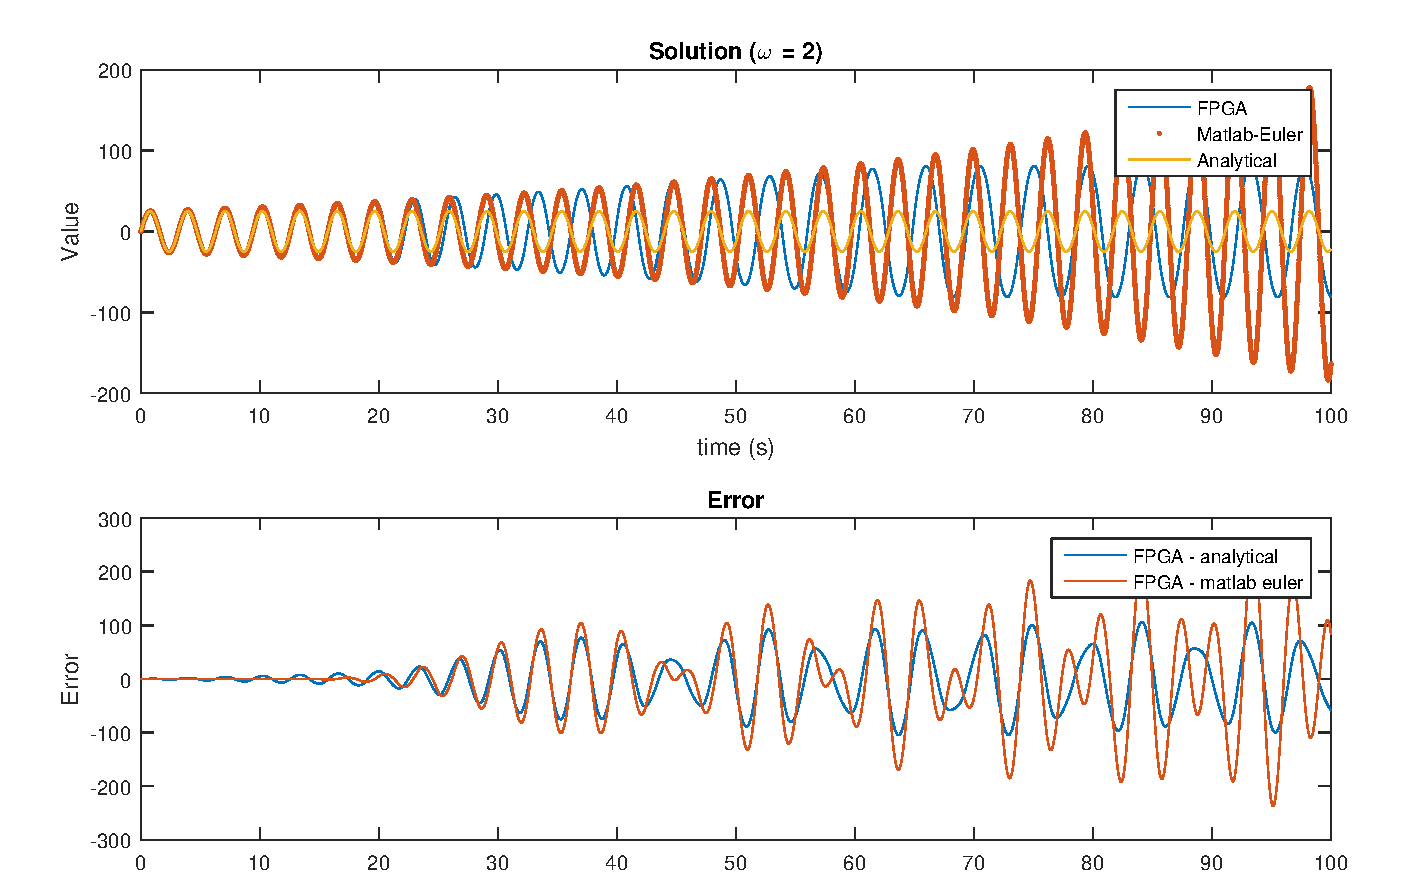
\includegraphics[width=\textwidth]{euler_o2_ts=0,01_os=1}
	\caption{Frequency shifting due to an insufficiently small time step (h = 0.01)}
	\label{f:euler_o2_ts=0,01_os=1}
\end{figure}

\begin{figure}[p]
	\centering
	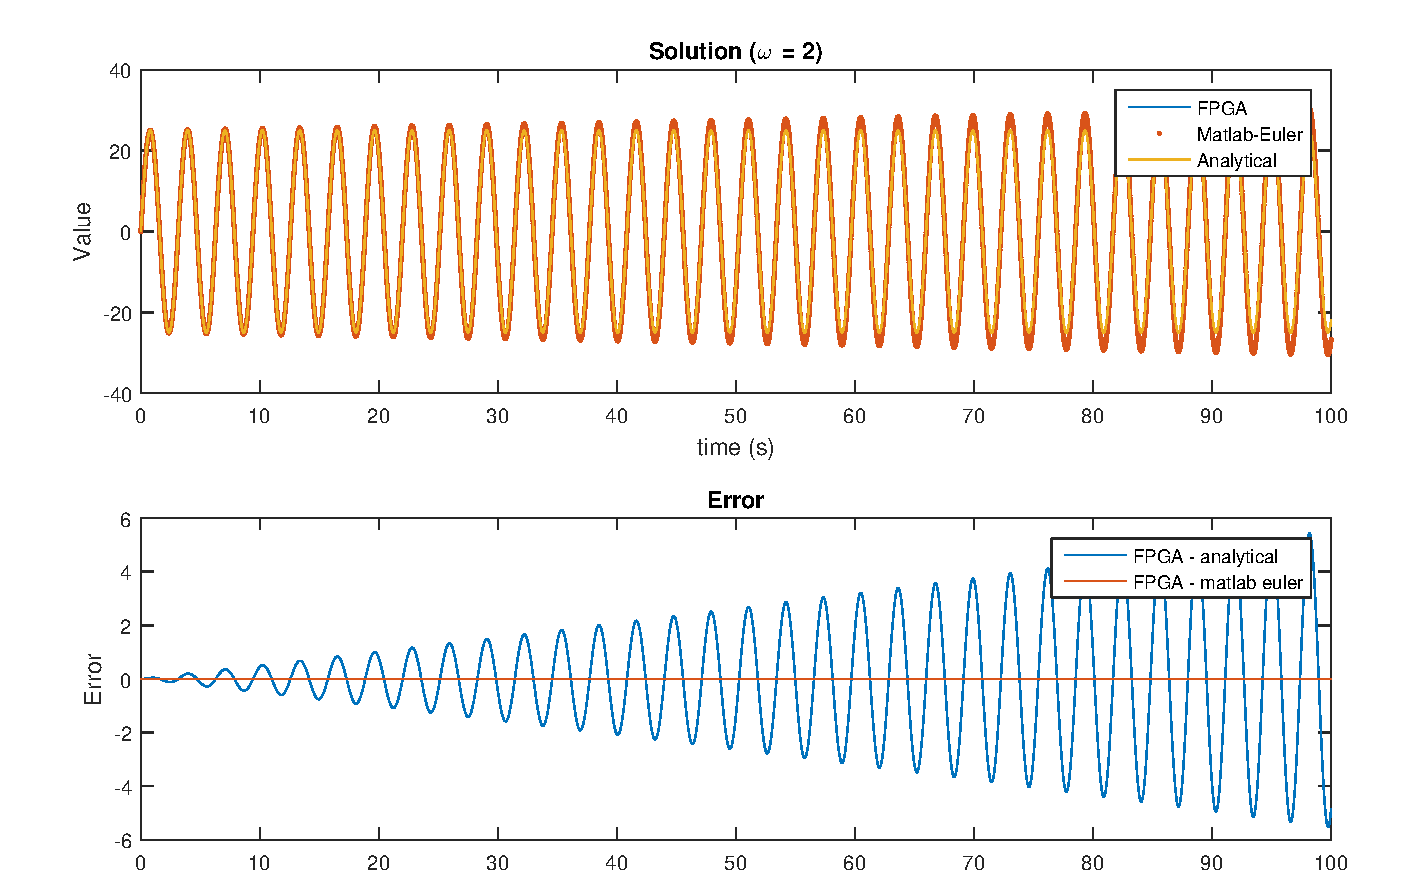
\includegraphics[width=0.95\textwidth]{euler_o2_ts=0,001_os=100}
	\caption{Relatively large time steps result in large errors in the long run (h=0.001)}
	\label{f:euler_o2_ts=0,001_os=100}
\end{figure}

\begin{figure}[p]
	\centering
	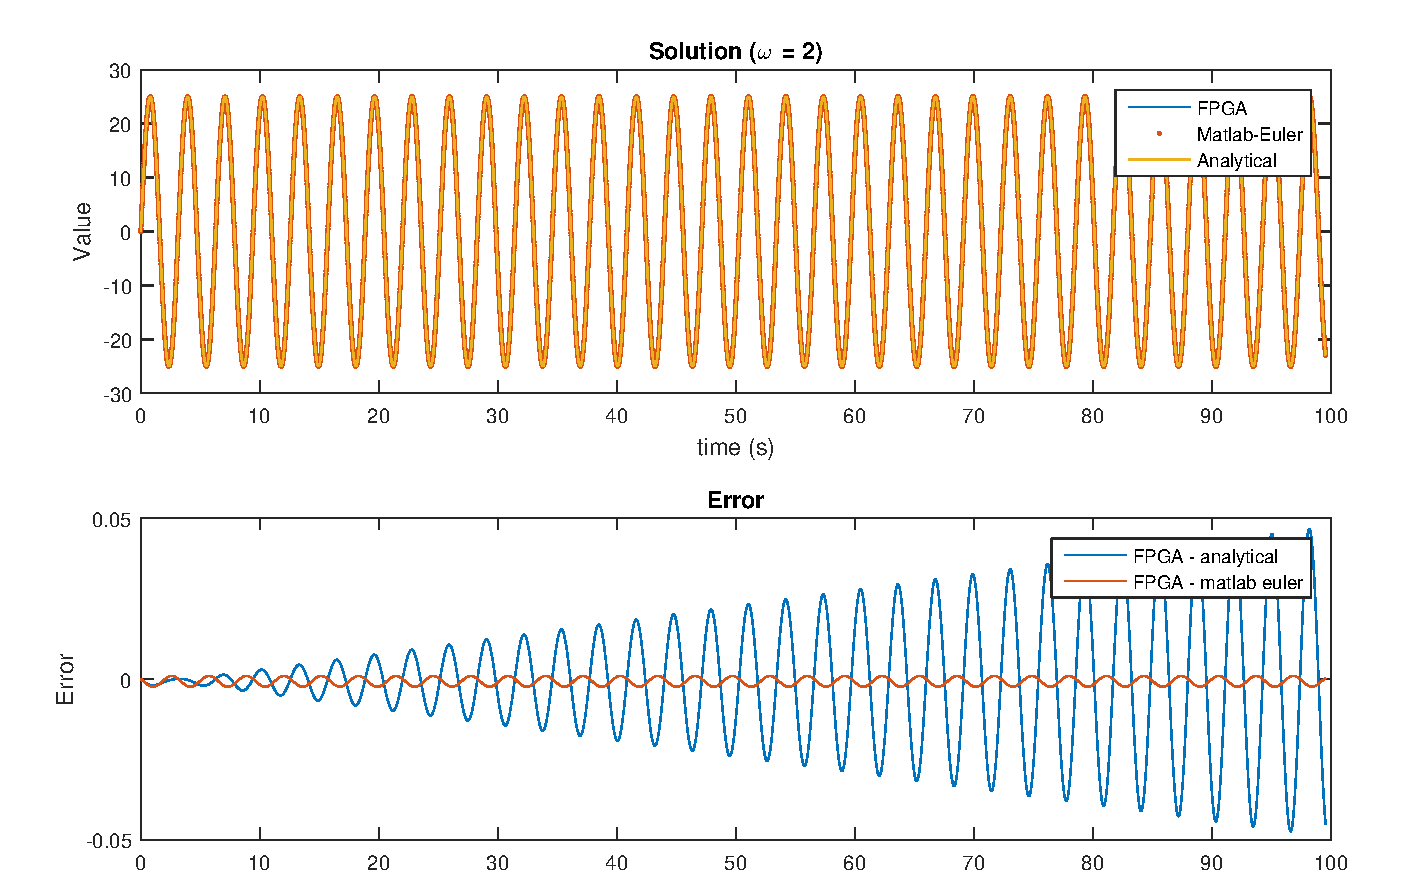
\includegraphics[width=0.95\textwidth]{euler_o2_ts=0,00001_os=1000}
	\caption{But a decrease in time step goes a long way in reducing the error. Note that the error due to the fixed point number representation starts to become significant again, in contrast to figure \ref{f:euler_o2_ts=0,001_os=100} (h = 1 \e{-5})}
	\label{f:euler_o2_ts=0,00001_os=1000}
\end{figure}

\section{Runge-Kutta (second order)}
The testing of the RK2 method uses a different matrix (equation \ref{eq:rk2matrix}) in order to verify the systems capability to correctly solve a system of 4, coupled, first order equations. The matrix has been generated randomly in \matlab{} under the constraint that all eigenvalues are negative. The reason as to why this property is necessary is, again, based on the fixed point number representation. Whenever one of the values (which could even occur internally as part of a vector dot product, invisible to interface) exceeds the allowed range, the result becomes invalid. If all elements in the vector described by the ODE tend towards zero, this problem is less likely to occur (but it might still happen whenever the initial conditions that have been chosen are too large). Furthermore, the added computational steps of RK2 compared to Euler's method have the effect that the time step becomes less important - for the entire range of possible time step values the results and errors are approximately the same (shown in figure \ref{f:rk2_ts=0,01_os=1} and \ref{f:rk2_ts=0,0000005_os=1000}). Lastly, in contrast to the FPGA solution, \matlab{} RK2 and ODE45 do remain close together which, once again, points in the direction of problems stemming from the fixed point numbers.

\begin{equation}
\label{eq:rk2matrix}
\vecb{x}' = \begin{bmatrix} 
2 & 3 & 2 & 0 \\
-5 & -5 & -3 & 1 \\
3 & -1 & -2 & -3 \\
4 & 2 & 2 & -3 \\
\end{bmatrix} \vecb{x} 
\hspace{20pt} \text{with} \hspace{20pt} 
\vecb{x}(t = 0) =\begin{bmatrix} 7 \\ 5 \\ 7 \\ 5 \end{bmatrix} 
\end{equation}

\begin{figure}[p]
	\centering
	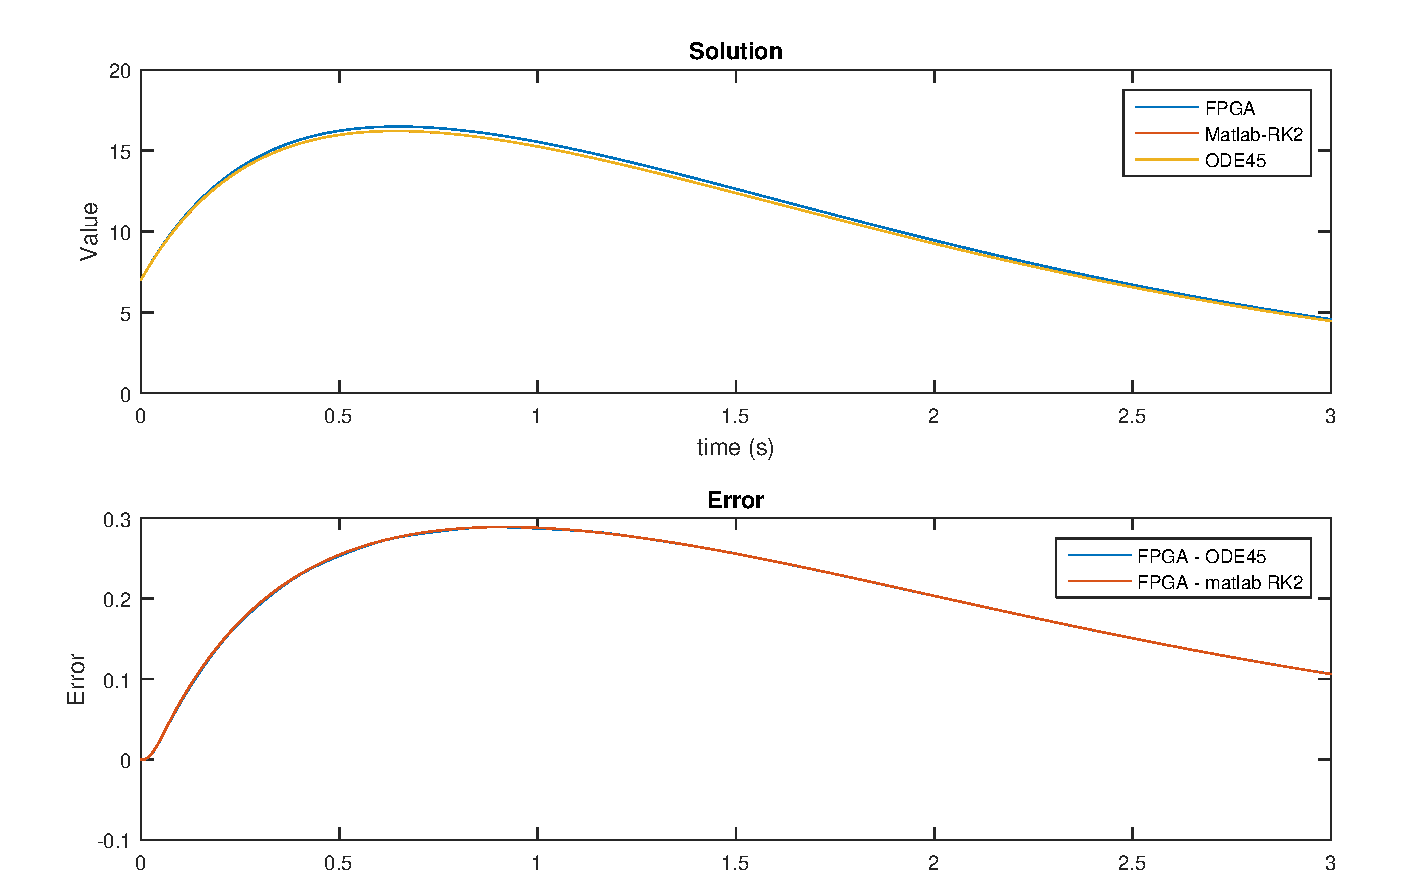
\includegraphics[width=0.95\textwidth]{rk2_ts=0,01_os=1}
	\caption{The largest possible time step has a maximum error of approximately 0.3, for both the comparison with the solution of ODE45 and \matlab{}s RK2 (h=0.01).}
	\label{f:rk2_ts=0,01_os=1}
\end{figure}

\begin{figure}[p]
	\centering
	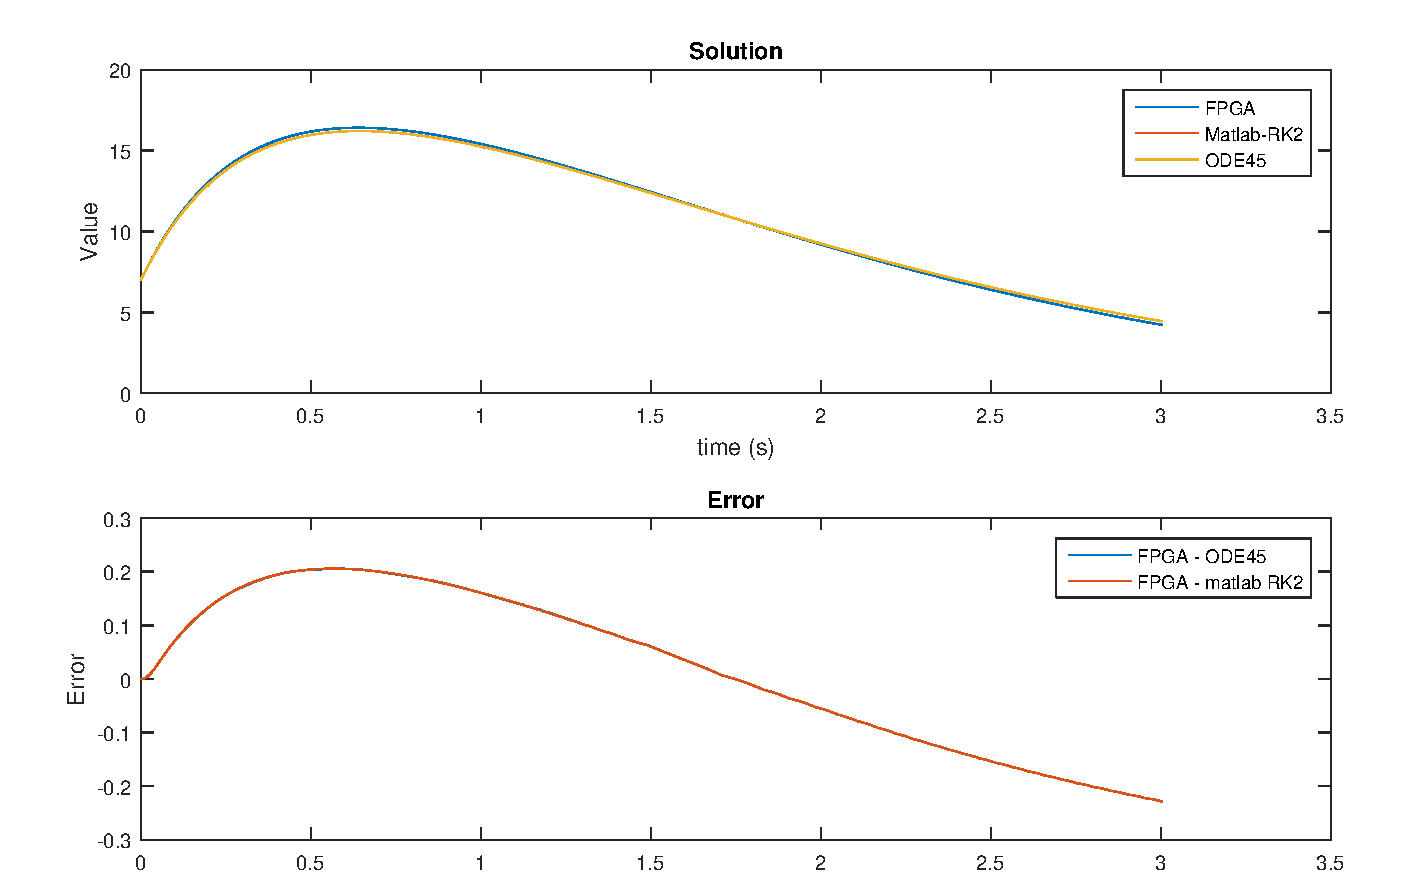
\includegraphics[width=0.95\textwidth]{rk2_ts=0,0000005_os=1000}
	\caption{Considering the other end of the spectrum regarding variety in time steps, the results do not differ significantly enough for the additional amount of work that has to be put in, a factor 20000 (h=5\e{-7}).}
	\label{f:rk2_ts=0,0000005_os=1000}
\end{figure}

\section{Runge-Kutta (fourth order)}
The RK4 integration scheme \footnote{Which took almost 22 hours or 78894 seconds to synthesize.} introduces even more computational steps, which leads to a faster overflow of the internal numbers. This means that at least one of the derivatives overflows almost immediately, which results in plots as shown in figure \ref{f:rk4_ts=0,00001_os=100}.


\begin{figure}[h]
	\centering
	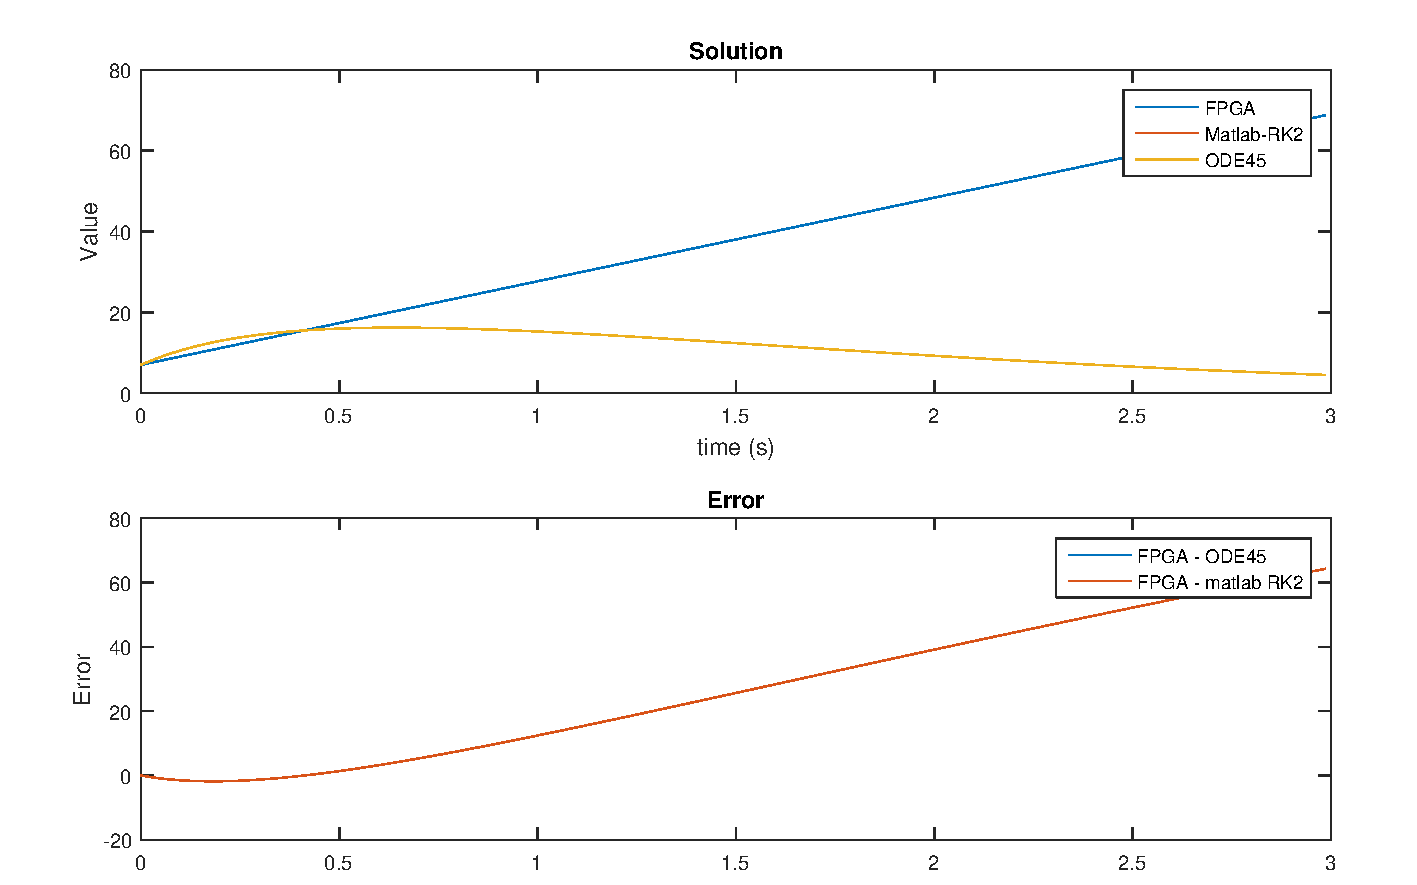
\includegraphics[width=\textwidth]{rk4_ts=0,00001_os=100}
	\caption{For every value of the time step the numbers overflow, causing derivatives to get stuck, resulting in straight lines instead of solutions to ODEs (h=1\e{-5}).}
	\label{f:rk4_ts=0,00001_os=100}
\end{figure}

\section{Euler revisited}
So far it appears that accuracy is inversely proportional to the complexity of the integration scheme, which leads to the question: What accuracy would Euler's method attain for equation \ref{eq:rk2matrix}? Indeed, as shown in figure \ref{f:euler_rv_ts=0,0001_os=10}, Euler's method only reaches maximum errors which are 2 orders of magnitude lower than the best values of the time step for RK2 and of course performs better than RK4 in this scenario. 

\section{Performance - add to conditions to appendix maybe?\textbf{}}
Performance is one of the main reasons why people use FPGAs over implementations in software and therefore one would expect that a properly written FPGA solution outperforms a CPU. The FPGA used for testing in this thesis is a Cyclone V, which, according to \cite{AlteraFPGA}, is meant for "your low-power, cost-sensitive design needs, enabling you to get to market faster". Furthermore, Altera offers two other FPGA families: Stratix and Arria, which both have mentions of delivering high or optimal performance. 

The FPGA runs at a clock speed of 50 MHz and it is capable of executing a single iteration of Euler's method per clock cycle. In theory this would mean that the FPGA is capable of 50\e{6} iterations per second. However, there is still quite some overhead stemming from the system handling the data input and output, which has to wait for the HPS to supply or request the proper information before the FPGA can move on with the computations.

\begin{table}
	\caption{Performance benchmarks: Euler's method}
	\label{t:perfomance}
	\begin{tabular}{l l l l l l}
		Device 	& Iterations& time (s)	& Output every	& Loop bound	& Iterations per second (\e{6}) \\  
		FPGA 	& 1\e{8} 	& 6,53		& 1.000			& 75			& 15,3 	\\
		FPGA 	& 1\e{8} 	& 4,61		& 10.000		& 750			& 21.7 	\\
		FPGA 	& 1\e{8} 	& 4,50		& 100.000		& 7.500			& 22,2 	\\
		FPGA 	& 1\e{8} 	& 4,36		& 100.000.000	& 7.500.000		& 22,9 	\\
		FPGA 	& 1\e{7} 	& 0,77		& 10.000.000	& 750.000		& 13,0 	\\
		FPGA 	& 1\e{6} 	& 0,42		& 1.000.000		& 75.000		& 2,3 	\\
		FPGA 	& 1\e{8} 	& 0,39		& 100.000		& 7.500			& 0,3 	\\
		CPU (i7)& 5\e{7} 	& 20,25		& 50.000.000	& -				& 2,5 	\\
		MATLAB 	& 1\e{7} 	& 303,83	& 10.000.000	& -				& 0,03	\\
	\end{tabular}
\end{table}

\begin{figure}[h!]
	\centering
	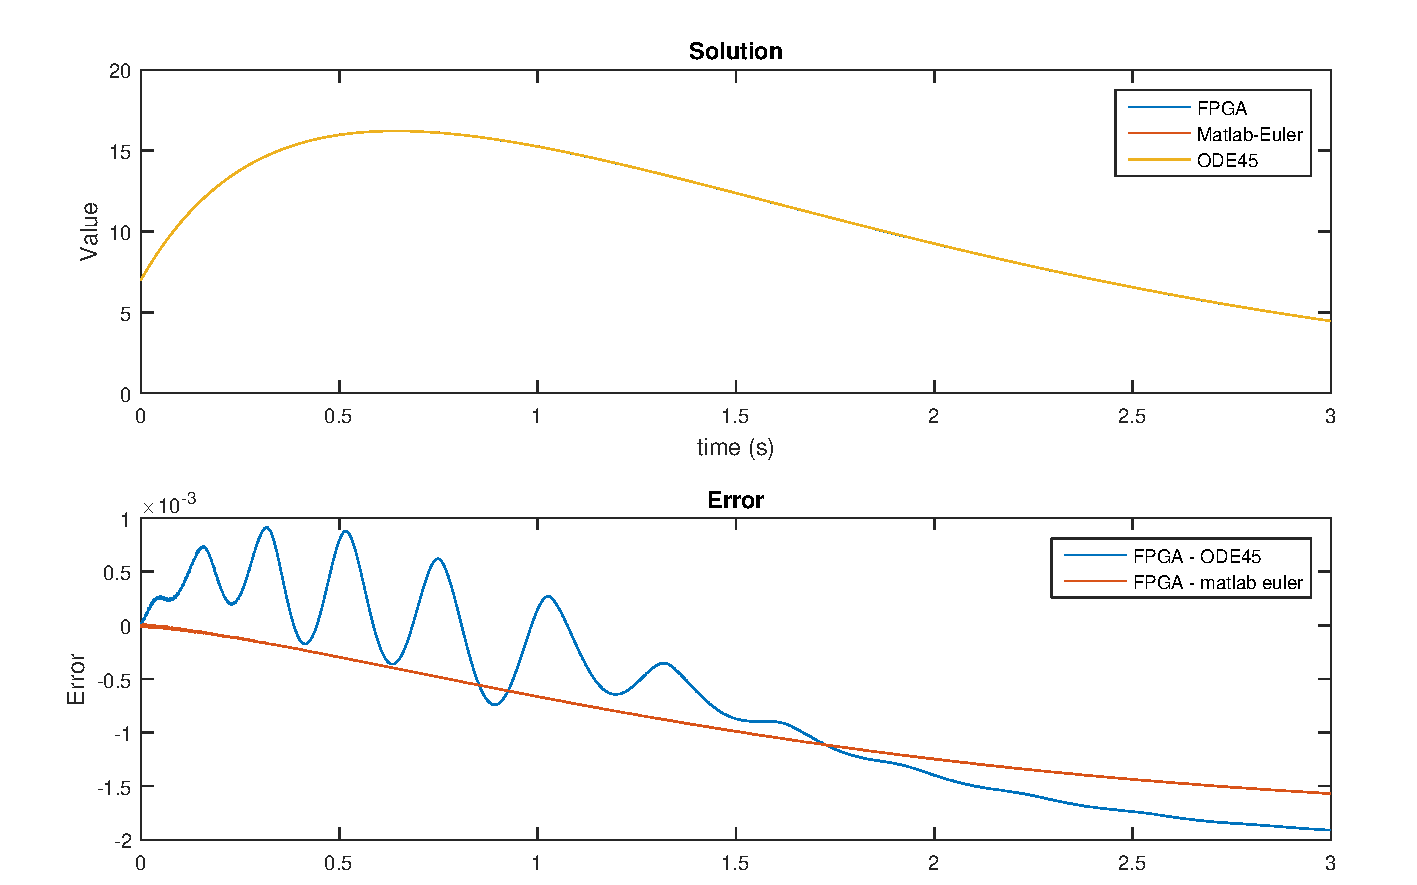
\includegraphics[width=0.9\textwidth]{euler_rv_ts=0,0001_os=10}
	\caption{Simplicity prevails: Euler's method attains better results than RK2 for all different time steps (h=1\e{-4}).}
	\label{f:euler_rv_ts=0,0001_os=10}
\end{figure}





\chapter{Conclusion}

\section{Keep in mind the number representation !! AVOID OVERFLOW}

%\include{Chapter6/chapter6}
%\include{Chapter7/chapter7}

%*******************************************************************************
%*********************************** First Chapter *****************************
%*******************************************************************************

\chapter{SAMPLE CODE - Getting started}  %Title of the First Chapter

\ifpdf
\graphicspath{{P2-Results/Figs/Raster/}{P2-Results/Figs/PDF/}{P2-Results/Figs/}}
\else
\graphicspath{{P2-Results/Figs/Vector/}{P2-Results/Figs/}}
\fi

\section{What is loren ipsum? Title with math \texorpdfstring{$\sigma$}{[sigma]}} %Section - 1.1 

Lorem Ipsum is simply dummy text of the printing and typesetting industry (see 
Section~\ref{section1.3}). Lorem Ipsum~\citep{Aup91} has been the industry's 
standard dummy text ever since the 1500s, when an unknown printer took a galley 
of type and scrambled it to make a type specimen book. It has survived not only 
five centuries, but also the leap into electronic typesetting, remaining 
essentially unchanged. It was popularised in the 1960s with the release of 
Letraset sheets containing Lorem Ipsum passages, and more recently with desktop 
publishing software like Aldus PageMaker including versions of Lorem 
Ipsum~\citep{AAB95,Con90,LM65}.

The most famous equation in the world: $E^2 = (m_0c^2)^2 + (pc)^2$, which is 
known as the \textbf{energy-mass-momentum} relation as an in-line equation.

A {\em \LaTeX{} class file}\index{\LaTeX{} class file@LaTeX class file} is a file, which holds style information for a particular \LaTeX{}.


\begin{align}
CIF: \hspace*{5mm}F_0^j(a) = \frac{1}{2\pi \iota} \oint_{\gamma} \frac{F_0^j(z)}{z - a} dz
\end{align}

\nomenclature[z-cif]{$CIF$}{Cauchy's Integral Formula}                                % first letter Z is for Acronyms 
\nomenclature[a-F]{$F$}{complex function}                                                   % first letter A is for Roman symbols
\nomenclature[g-p]{$\pi$}{ $\simeq 3.14\ldots$}                                             % first letter G is for Greek Symbols
\nomenclature[g-i]{$\iota$}{unit imaginary number $\sqrt{-1}$}                      % first letter G is for Greek Symbols
\nomenclature[g-g]{$\gamma$}{a simply closed curve on a complex plane}  % first letter G is for Greek Symbols
\nomenclature[x-i]{$\oint_\gamma$}{integration around a curve $\gamma$} % first letter X is for Other Symbols
\nomenclature[r-j]{$j$}{superscript index}                                                       % first letter R is for superscripts
\nomenclature[s-0]{$0$}{subscript index}                                                        % first letter S is for subscripts


%********************************** %Second Section  *************************************
\section{Why do we use loren ipsum?} %Section - 1.2


It is a long established fact that a reader will be distracted by the readable content of a page when looking at its layout. The point of using Lorem Ipsum is that it has a more-or-less normal distribution of letters, as opposed to using `Content here, content here', making it look like readable English. Many desktop publishing packages and web page editors now use Lorem Ipsum as their default model text, and a search for `lorem ipsum' will uncover many web sites still in their infancy. Various versions have evolved over the years, sometimes by accident, sometimes on purpose (injected humour and the like).

%********************************** % Third Section  *************************************
\section{Where does it come from?}  %Section - 1.3 
\label{section1.3}

Contrary to popular belief, Lorem Ipsum is not simply random text. It has roots in a piece of classical Latin literature from 45 BC, making it over 2000 years old. Richard McClintock, a Latin professor at Hampden-Sydney College in Virginia, looked up one of the more obscure Latin words, consectetur, from a Lorem Ipsum passage, and going through the cites of the word in classical literature, discovered the undoubtable source. Lorem Ipsum comes from sections 1.10.32 and 1.10.33 of "de Finibus Bonorum et Malorum" (The Extremes of Good and Evil) by Cicero, written in 45 BC. This book is a treatise on the theory of ethics, very popular during the Renaissance. The first line of Lorem Ipsum, "Lorem ipsum dolor sit amet..", comes from a line in section 1.10.32.

The standard chunk of Lorem Ipsum used since the 1500s is reproduced below for those interested. Sections 1.10.32 and 1.10.33 from ``de Finibus Bonorum et Malorum" by Cicero are also reproduced in their exact original form, accompanied by English versions from the 1914 translation by H. Rackham

``Lorem ipsum dolor sit amet, consectetur adipisicing elit, sed do eiusmod tempor incididunt ut labore et dolore magna aliqua. Ut enim ad minim veniam, quis nostrud exercitation ullamco laboris nisi ut aliquip ex ea commodo consequat. Duis aute irure dolor in reprehenderit in voluptate velit esse cillum dolore eu fugiat nulla pariatur. Excepteur sint occaecat cupidatat non proident, sunt in culpa qui officia deserunt mollit anim id est laborum."

Section 1.10.32 of ``de Finibus Bonorum et Malorum", written by Cicero in 45 BC: ``Sed ut perspiciatis unde omnis iste natus error sit voluptatem accusantium doloremque laudantium, totam rem aperiam, eaque ipsa quae ab illo inventore veritatis et quasi architecto beatae vitae dicta sunt explicabo. Nemo enim ipsam voluptatem quia voluptas sit aspernatur aut odit aut fugit, sed quia consequuntur magni dolores eos qui ratione voluptatem sequi nesciunt. Neque porro quisquam est, qui dolorem ipsum quia dolor sit amet, consectetur, adipisci velit, sed quia non numquam eius modi tempora incidunt ut labore et dolore magnam aliquam quaerat voluptatem. Ut enim ad minima veniam, quis nostrum exercitationem ullam corporis suscipit laboriosam, nisi ut aliquid ex ea commodi consequatur? Quis autem vel eum iure reprehenderit qui in ea voluptate velit esse quam nihil molestiae consequatur, vel illum qui dolorem eum fugiat quo voluptas nulla pariatur?"

1914 translation by H. Rackham: ``But I must explain to you how all this mistaken idea of denouncing pleasure and praising pain was born and I will give you a complete account of the system, and expound the actual teachings of the great explorer of the truth, the master-builder of human happiness. No one rejects, dislikes, or avoids pleasure itself, because it is pleasure, but because those who do not know how to pursue pleasure rationally encounter consequences that are extremely painful. Nor again is there anyone who loves or pursues or desires to obtain pain of itself, because it is pain, but because occasionally circumstances occur in which toil and pain can procure him some great pleasure. To take a trivial example, which of us ever undertakes laborious physical exercise, except to obtain some advantage from it? But who has any right to find fault with a man who chooses to enjoy a pleasure that has no annoying consequences, or one who avoids a pain that produces no resultant pleasure?"

Section 1.10.33 of ``de Finibus Bonorum et Malorum", written by Cicero in 45 BC: ``At vero eos et accusamus et iusto odio dignissimos ducimus qui blanditiis praesentium voluptatum deleniti atque corrupti quos dolores et quas molestias excepturi sint occaecati cupiditate non provident, similique sunt in culpa qui officia deserunt mollitia animi, id est laborum et dolorum fuga. Et harum quidem rerum facilis est et expedita distinctio. Nam libero tempore, cum soluta nobis est eligendi optio cumque nihil impedit quo minus id quod maxime placeat facere possimus, omnis voluptas assumenda est, omnis dolor repellendus. Temporibus autem quibusdam et aut officiis debitis aut rerum necessitatibus saepe eveniet ut et voluptates repudiandae sint et molestiae non recusandae. Itaque earum rerum hic tenetur a sapiente delectus, ut aut reiciendis voluptatibus maiores alias consequatur aut perferendis doloribus asperiores repellat."

1914 translation by H. Rackham: ``On the other hand, we denounce with righteous indignation and dislike men who are so beguiled and demoralized by the charms of pleasure of the moment, so blinded by desire, that they cannot foresee the pain and trouble that are bound to ensue; and equal blame belongs to those who fail in their duty through weakness of will, which is the same as saying through shrinking from toil and pain. These cases are perfectly simple and easy to distinguish. In a free hour, when our power of choice is untrammelled and when nothing prevents our being able to do what we like best, every pleasure is to be welcomed and every pain avoided. But in certain circumstances and owing to the claims of duty or the obligations of business it will frequently occur that pleasures have to be repudiated and annoyances accepted. The wise man therefore always holds in these matters to this principle of selection: he rejects pleasures to secure other greater pleasures, or else he endures pains to avoid worse pains."

\section[Short title]{Reasonably long section title}

% Uncomment this line, when you have siunitx package loaded.
%The SI Units for dynamic viscosity is \si{\newton\second\per\metre\squared}.
I'm going to randomly include a picture Figure~\ref{fig:minion}.


If you have trouble viewing this document contact Krishna at: \href{mailto:kks32@cam.ac.uk}{kks32@cam.ac.uk} or raise an issue at \url{https://github.com/kks32/phd-thesis-template/}


\begin{figure}[htbp!] 
	\centering    
	
\includegraphics[width=1.0\textwidth]{minion}
	\caption[Minion]{This is just a long figure caption for the minion in Despicable Me from Pixar}
	\label{fig:minion}
\end{figure}


\section*{Enumeration}
\begin{enumerate}
	\item The first topic is dull
	\item The second topic is duller
	\begin{enumerate}
		\item The first subtopic is silly
		\item The second subtopic is stupid
	\end{enumerate}
	\item The third topic is the dullest
\end{enumerate}

\section*{itemize}
\begin{itemize}
	\item The first topic is dull
	\item The second topic is duller
	\begin{itemize}
		\item The first subtopic is silly
		\item The second subtopic is stupid
	\end{itemize}
	\item The third topic is the dullest
\end{itemize}

\section*{description}
\begin{description}
	\item[The first topic] is dull
	\item[The second topic] is duller
	\begin{description}
		\item[The first subtopic] is silly
		\item[The second subtopic] is stupid
	\end{description}
	\item[The third topic] is the dullest
\end{description}


\clearpage

\tochide\section{Hidden section}
\textbf{Lorem ipsum dolor sit amet}, \textit{consectetur adipiscing elit}. In magna nisi, aliquam id blandit id, congue ac est. Fusce porta consequat leo. Proin feugiat at felis vel consectetur. Ut tempus ipsum sit amet congue posuere. Nulla varius rutrum quam. Donec sed purus luctus, faucibus velit id, ultrices sapien. Cras diam purus, tincidunt eget tristique ut, egestas quis nulla. Curabitur vel iaculis lectus. Nunc nulla urna, ultrices et eleifend in, accumsan ut erat. In ut ante leo. Aenean a lacinia nisl, sit amet ullamcorper dolor. Maecenas blandit, tortor ut scelerisque congue, velit diam volutpat metus, sed vestibulum eros justo ut nulla. Etiam nec ipsum non enim luctus porta in in massa. Cras arcu urna, malesuada ut tellus ut, pellentesque mollis risus.Morbi vel tortor imperdiet arcu auctor mattis sit amet eu nisi. Nulla gravida urna vel nisl egestas varius. Aliquam posuere ante quis malesuada dignissim. Mauris ultrices tristique eros, a dignissim nisl iaculis nec. Praesent dapibus tincidunt mauris nec tempor. Curabitur et consequat nisi. Quisque viverra egestas risus, ut sodales enim blandit at. Mauris quis odio nulla. Cras euismod turpis magna, in facilisis diam congue non. Mauris faucibus nisl a orci dictum, et tempus mi cursus.

Etiam elementum tristique lacus, sit amet eleifend nibh eleifend sed \footnote{My footnote goes blah blah blah! \dots}. Maecenas dapibu augue ut urna malesuada, non tempor nibh mollis. Donec sed sem sollicitudin, convallis velit aliquam, tincidunt diam. In eu venenatis lorem. Aliquam non augue porttitor tellus faucibus porta et nec ante. Proin sodales, libero vitae commodo sodales, dolor nisi cursus magna, non tincidunt ipsum nibh eget purus. Nam rutrum tincidunt arcu, tincidunt vulputate mi sagittis id. Proin et nisi nec orci tincidunt auctor et porta elit. Praesent eu dolor ac magna cursus euismod. Integer non dictum nunc.


\begin{landscape}
	
	\section*{Subplots}
	I can cite Wall-E (see Fig.~\ref{fig:WallE}) and Minions in despicable me (Fig.~\ref{fig:Minnion}) or I can cite the whole figure as Fig.~\ref{fig:animations}
	
	\begin{figure}
		\centering
		\begin{subfigure}[b]{0.3\textwidth}
			
\includegraphics[width=\textwidth]{TomandJerry}
			\caption{Tom and Jerry}
			\label{fig:TomJerry}   
		\end{subfigure}             
		\begin{subfigure}[b]{0.3\textwidth}
			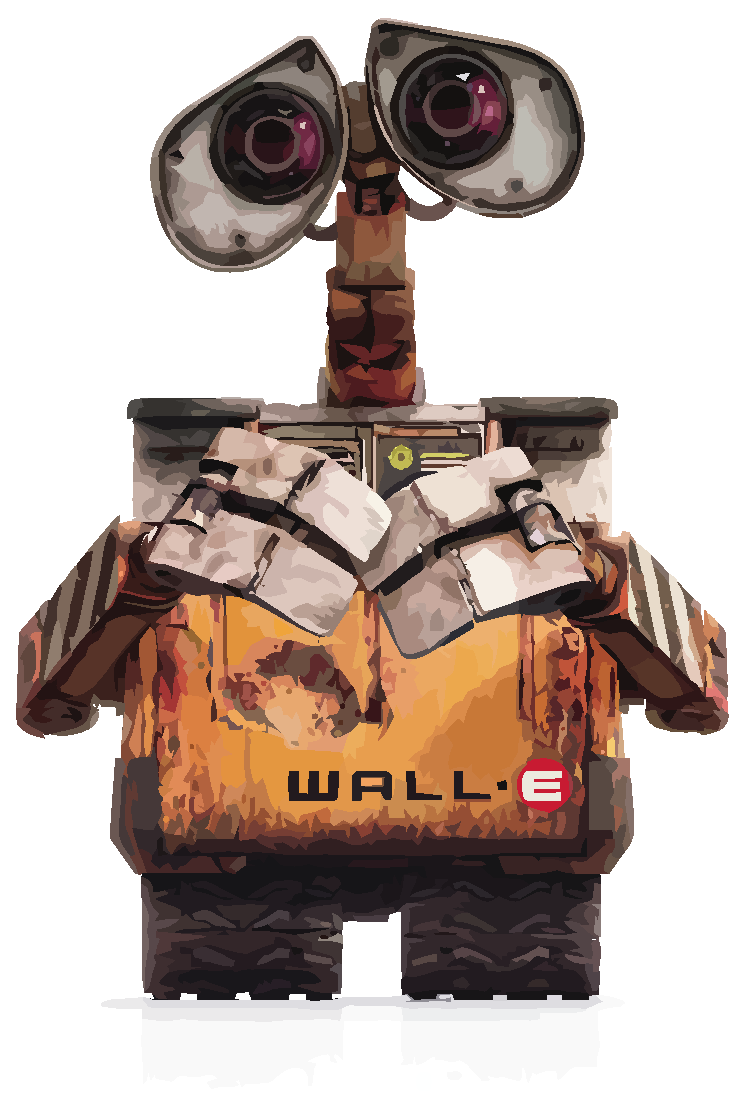
\includegraphics[width=\textwidth]{WallE}
			\caption{Wall-E}
			\label{fig:WallE}
		\end{subfigure}             
		\begin{subfigure}[b]{0.3\textwidth}
			
\includegraphics[width=\textwidth]{minion}
			\caption{Minions}
			\label{fig:Minnion}
		\end{subfigure}
		\caption{Best Animations}
		\label{fig:animations}
	\end{figure}
	

\end{landscape}

\section{First section of the third chapter}
And now I begin my third chapter here \dots

And now to cite some more people~\citet{Rea85,Ancey1996}

\subsection{First subsection in the first section}
\dots and some more 

\subsection{Second subsection in the first section}
\dots and some more \dots

\subsubsection{First subsub section in the second subsection}
\dots and some more in the first subsub section otherwise it all looks the same
doesn't it? well we can add some text to it \dots

\subsection{Third subsection in the first section}
\dots and some more \dots

\subsubsection{First subsub section in the third subsection}
\dots and some more in the first subsub section otherwise it all looks the same
doesn't it? well we can add some text to it and some more and some more and
some more and some more and some more and some more and some more \dots

\subsubsection{Second subsub section in the third subsection}
\dots and some more in the first subsub section otherwise it all looks the same
doesn't it? well we can add some text to it \dots

\section{Second section of the third chapter}
and here I write more \dots

\section{The layout of formal tables}
This section has been modified from ``Publication quality tables in \LaTeX*''
by Simon Fear.

The layout of a table has been established over centuries of experience and 
should only be altered in extraordinary circumstances. 

When formatting a table, remember two simple guidelines at all times:

\begin{enumerate}
	\item Never, ever use vertical rules (lines).
	\item Never use double rules.
\end{enumerate}

These guidelines may seem extreme but I have
never found a good argument in favour of breaking them. For
example, if you feel that the information in the left half of
a table is so different from that on the right that it needs
to be separated by a vertical line, then you should use two
tables instead. Not everyone follows the second guideline:

There are three further guidelines worth mentioning here as they
are generally not known outside the circle of professional
typesetters and subeditors:

\begin{enumerate}\setcounter{enumi}{2}
	\item Put the units in the column heading (not in the body of
	the table).
	\item Always precede a decimal point by a digit; thus 0.1
	{\em not} just .1.
	\item Do not use `ditto' signs or any other such convention to
	repeat a previous value. In many circumstances a blank
	will serve just as well. If it won't, then repeat the value.
\end{enumerate}

A frequently seen mistake is to use `\textbackslash begin\{center\}' \dots `\textbackslash end\{center\}' inside a figure or table environment. This center environment can cause additional vertical space. If you want to avoid that just use `\textbackslash centering'


\begin{table}
	\caption{A badly formatted table}
	\centering
	\label{table:bad_table}
	\begin{tabular}{|l|c|c|c|c|}
		\hline 
		& \multicolumn{2}{c}{Species I} & \multicolumn{2}{c|}{Species II} \\ 
		\hline
		Dental measurement  & mean & SD  & mean & SD  \\ \hline 
		\hline
		I1MD & 6.23 & 0.91 & 5.2  & 0.7  \\
		\hline 
		I1LL & 7.48 & 0.56 & 8.7  & 0.71 \\
		\hline 
		I2MD & 3.99 & 0.63 & 4.22 & 0.54 \\
		\hline 
		I2LL & 6.81 & 0.02 & 6.66 & 0.01 \\
		\hline 
		CMD & 13.47 & 0.09 & 10.55 & 0.05 \\
		\hline 
		CBL & 11.88 & 0.05 & 13.11 & 0.04\\ 
		\hline 
	\end{tabular}
\end{table}

\begin{table}
	\caption{A nice looking table}
	\centering
	\label{table:nice_table}
	\begin{tabular}{l c c c c}
		\hline 
		\multirow{2}{*}{Dental measurement} & \multicolumn{2}{c}{Species I} & \multicolumn{2}{c}{Species II} \\ 
		\cline{2-5}
		& mean & SD  & mean & SD  \\ 
		\hline
		I1MD & 6.23 & 0.91 & 5.2  & 0.7  \\
		
		I1LL & 7.48 & 0.56 & 8.7  & 0.71 \\
		
		I2MD & 3.99 & 0.63 & 4.22 & 0.54 \\
		
		I2LL & 6.81 & 0.02 & 6.66 & 0.01 \\
		
		CMD & 13.47 & 0.09 & 10.55 & 0.05 \\
		
		CBL & 11.88 & 0.05 & 13.11 & 0.04\\ 
		\hline 
	\end{tabular}
\end{table}


\begin{table}
	\caption{Even better looking table using booktabs}
	\centering
	\label{table:good_table}
	\begin{tabular}{l c c c c}
		\toprule
		\multirow{2}{*}{Dental measurement} & \multicolumn{2}{c}{Species I} & \multicolumn{2}{c}{Species II} \\ 
		\cmidrule{2-5}
		& mean & SD  & mean & SD  \\ 
		\midrule
		I1MD & 6.23 & 0.91 & 5.2  & 0.7  \\
		
		I1LL & 7.48 & 0.56 & 8.7  & 0.71 \\
		
		I2MD & 3.99 & 0.63 & 4.22 & 0.54 \\
		
		I2LL & 6.81 & 0.02 & 6.66 & 0.01 \\
		
		CMD & 13.47 & 0.09 & 10.55 & 0.05 \\
		
		CBL & 11.88 & 0.05 & 13.11 & 0.04\\ 
		\bottomrule
	\end{tabular}
\end{table}


% ********************************** Back Matter *******************************
% Backmatter should be commented out, if you are using appendices after References
%\backmatter

% ********************************** Bibliography ******************************
\begin{spacing}{0.9}

% To use the conventional natbib style referencing
% Bibliography style previews: http://nodonn.tipido.net/bibstyle.php
% Reference styles: http://sites.stat.psu.edu/~surajit/present/bib.htm

\bibliographystyle{apalike}
%\bibliographystyle{plainnat} % use this to have URLs listed in References
\cleardoublepage
\bibliography{References/references} % Path to your References.bib file


% If you would like to use BibLaTeX for your references, pass `custombib' as
% an option in the document class. The location of 'reference.bib' should be
% specified in the preamble.tex file in the custombib section.
% Comment out the lines related to natbib above and uncomment the following line.

%\printbibliography[heading=bibintoc, title={References}]


\end{spacing}

% ********************************** Appendices ********************************

\begin{appendices} % Using appendices environment for more functunality

% ******************************* Thesis Appendix A ****************************
\chapter{Haskell source code for numerical solutions of ODEs} 
\label{app:haskellsolver}
\lstset{style=haskellStyle}

\lstinputlisting[caption=Solver.hs]{../haskell/Solver.hs}
\lstinputlisting[caption=SolverTypes.hs]{../haskell/SolverTypes.hs}
\lstinputlisting[caption=SolverEquations.hs]{../haskell/SolverEquations.hs}

\lstinputlisting[caption=SolverPresets.hs]{../haskell/SolverPresets.hs}
\lstinputlisting[caption=SolverHelper.hs]{../haskell/SolverHelper.hs}
\lstinputlisting[caption=SolverPlotter.hs]{../haskell/SolverPlotter.hs}
% ******************************* Thesis Appendix B ********************************

\chapter{Installing the CUED class file}

\LaTeX.cls files can be accessed system-wide when they are placed in the
<texmf>/tex/latex directory, where <texmf> is the root directory of the user’s \TeX installation. On systems that have a local texmf tree (<texmflocal>), which
may be named ``texmf-local'' or ``localtexmf'', it may be advisable to install packages in <texmflocal>, rather than <texmf> as the contents of the former, unlike that of the latter, are preserved after the \LaTeX system is reinstalled and/or upgraded.

It is recommended that the user create a subdirectory <texmf>/tex/latex/CUED for all CUED related \LaTeX class and package files. On some \LaTeX systems, the directory look-up tables will need to be refreshed after making additions or deletions to the system files. For \TeX Live systems this is accomplished via executing ``texhash'' as root. MIK\TeX users can run ``initexmf -u'' to accomplish the same thing.

Users not willing or able to install the files system-wide can install them in their personal directories, but will then have to provide the path (full or relative) in addition to the filename when referring to them in \LaTeX.



\end{appendices}

% *************************************** Index ********************************
\printthesisindex % If index is present

\end{document}
